\documentclass[letterpaper,12pt]{article}

\usepackage{tabularx} % extra features for tabular environment
\usepackage{amsmath}  % improve math presentation
\usepackage{graphicx} % takes care of graphic including machinery
\usepackage[margin=1in,letterpaper]{geometry} % decreases margins
\usepackage{cite} % takes care of citations
\usepackage[final]{hyperref} % adds hyper links inside the generated pdf file
\usepackage{ctex}
\usepackage{titlesec}
\usepackage{CJKutf8, CJK}
\usepackage{makecell}                 % 三线表-竖线
\usepackage{booktabs}                 % 三线表-短细横线
% \usepackage{natbib}
\usepackage{graphicx}				  % 表格单元格逆时针
\usepackage{multirow}				  % 合并单元格
\usepackage{array}
\usepackage{amssymb}				  % 勾
\usepackage{amsmath}
\usepackage{longtable}                % 导入 longtable 宏包,表格自动换行
\usepackage{caption}
\usepackage{subcaption}               % 设置子图
\usepackage{color}					  % 文本颜色包
\usepackage{xcolor}
\usepackage{bbm}					  % 输入指示函数
\usepackage{tablefootnote}			  % 表格注释

\hypersetup{
	colorlinks=true,       % false: boxed links; true: colored links
	linkcolor=blue,        % color of internal links
	citecolor=blue,        % color of links to bibliography
	filecolor=magenta,     % color of file links
	urlcolor=blue         
}
%++++++++++++++++++++++++++++++++++++++++
\titleformat{\section}{\Large\bfseries\songti}{\thesection}{1em}{}
\titleformat{\subsection}{\large\bfseries\songti}{\thesubsection}{1em}{}
\titleformat{\subsubsection}{\normalsize\bfseries\songti}{\thesubsubsection}{1em}{}

\begin{document}
	
	
	\title{\songti \zihao{4}4月28日-5月5日工作汇报}
	\author{\textrm{Ku Jui}}
	\date{\textrm{May 2023}}
	\maketitle
	
	\renewcommand{\figurename}{Figure} % 可以重新定义abstract,因为ctex会覆盖thebibliography
% 	\begin{abstract}
%		In this experiment we studied a very important physical effect by measuring the
%		dependence of a quantity $V$ of the quantity $X$ for two different sample
%		temperatures.  Our experimental measurements confirmed the quadratic dependence
%		$V = kX^2$ predicted by Someone's first law. The value of the mystery parameter
%		$k = 15.4\pm 0.5$~s was extracted from the fit. This value is
%		not consistent with the theoretically predicted $k_{theory}=17.34$~s. We attribute %this
%		discrepancy to low efficiency of our $V$-detector.
%	\end{abstract}
	\renewcommand{\contentsname}{Contents}
	
	\tableofcontents  % 自动生成目录
	
	\section{文献阅读}

	\subsection{Pre-knowledge}
	
	经典的Retinex理论模拟了人眼颜色感知,它假设观测图像可以被分解为两种成分:
	Reflectance与Illumination。假设$S$表示观测图像,它可以被分解为:$$S = R \circ I$$

	其中,$R$表示反射图,$I$表示亮度图, $\circ$表示点乘操作。反射图描述了观测目标的固有属性,它可以被视作常量且与光照无关;亮度图表示了目标的不同光照。低光图像存在暗光与不平衡的亮度分布。
	
	在传统方法中,Single Scale Retinex, SSR通过高斯滤波为亮度图添加平滑性作为最早期的尝试;MSR, MSRCR通过添加多尺度高斯滤波与颜色还原对SSR进行了拓展。关于更多相关技术可以参考:Retinex Image Processing.

	在深度学习方法中,已有诸多方法尝试将Retinex理论与深度网络相结合,在降低学习难度的同时提升算法性能,如RetinexNet。
	
	\subsection{(综述2021.04)Lighting the darkness in the deep learning era}
	
	\subsubsection{背景}
	
	该领域的近期进展主要由深度学习方法(包含不同学习策略、网络架构、损失函数、训练数据等)主导。
	
	\subsubsection{介绍}
	
	这篇文章从低光图像增强的数据集、网络架构、损失函数、学习机制等不同角度对其进行了系统性的综述;
	
	(1) 为评估不同方法的泛化性与鲁棒性还提出了一个大尺度低光图像数据集;
	
	(2) 这篇文章首个系统而全面的对基于深度学习的LLIE方法进行了综述;
	
	(3) 这篇文章提出一个包含不同收集在不同亮度条件下锁舌的大尺度低光图像/视频数据集并用于评估现有方法的泛化性能;
	
	(4) 这篇文章提供了一个包含多种主流LLE方法的在线平台,它可以让用户以更友好交互方式重现不同方法的效果。
	
	
	\subsubsection{细节}
	
	\renewcommand{\tablename}{Table}
	
	\begin{table}[!htbp]
		\centering
		\tiny
		\resizebox{\textwidth}{!}{ %按照宽度调整调整表格大小
		\begin{tabular}{m{0.01cm}|>{\centering\arraybackslash}m{1.45cm}|>{\centering\arraybackslash}m{1.0cm}|>{\centering\arraybackslash}m{2.6cm}|>{\centering\arraybackslash}m{3.1cm}|>{\centering\arraybackslash}m{3cm}|>{\centering\arraybackslash}m{2.4cm}|>{\centering\arraybackslash}m{2.4cm}|>{\centering\arraybackslash}m{0.9cm}|>{\centering\arraybackslash}m{1.4cm}|>{\centering\arraybackslash}m{1cm}|}
			
			\hline
			
			& \textbf{Method} & \textbf{Learning} & \textbf{Network Structure} & \textbf{Loss Function} & \textbf{Training Data} & \textbf{Testing Data} & \makecell{\textbf{Evaluation Metric}} & \textbf{Format} & \textbf{Platform} & \textbf{Retinex} \\
			
			\hline
			
			\multirowcell{1}{\makecell{\centering \rotatebox{90}{\textbf{2017}}}} & LLNet & SL & SSDA &  SRR loss & simulated by Gamma Correction \& Gaussian Noise & simulated self-selected & PSNR SSIM & RGB & Theano &  \\
			
			\hline
			
			\multirowcell{6}{\makecell{\centering \rotatebox{90}{\textbf{2018}}}} & LightenNet & SL &  four layers & $L_2$ loss & simulated by random illumination values & simulated self-selected & \makecell{PSNR MAE \\ SSIM User Study} & RGB & Caffe MATLAB & \checkmark \\
			
			& Retinex-Net  & SL & multi-scale network & \makecell{$L_1$ loss \\ invariable reflectance loss \\ smoothness loss} & LOL simulated by adjusting histogram & self-selected & - & RGB & TensorFlow & \ \checkmark \\
			
			& MBLLEN & SL & multi-branch fusion & SSIM loss perceptual loss region loss & simulated by Gamma Correction \& Poisson Noise & simulated self-selected & \makecell{PSNR SSIM \\ AB VIF \\ LOE TOMI} & RGB & TensorFlow &  \\
			
			& SCIE & SL & frequency decomposition & \makecell{$L_2$ loss \\ $L_1$ loss \\ SSIM loss} & SCIE & SCIE & PSNR FSIM \qquad Runtime FLOPs & RGB & Caffe MATLAB &  \\
			
			& Chen et al. & SL & U-Net & $L_1$ loss & SID & SID & PSNR SSIM & Raw & TensorFlow &  \\
			
			& Deepexposure & RL & policy network GAN & deterministic policy gradient adversarial loss & MIT-Adobe FiveK & MIT-Adobe FiveK & PSNR SSIM & Raw & TensorFlow &  \\
			
			\hline
			
			\multirowcell{8}{\makecell{\centering \rotatebox{90}{\textbf{2019}\qquad\qquad \qquad\qquad\qquad}}} & Chen et al. & SL & siamese network & $L_1$ loss self-consistency loss & DRV & DRV & \makecell{PSNR SSIM \\ MAE} & Raw & TensorFlow &  \\

			
			& Jiang and Zheng & SL & 3D U-Net & \makecell{$L_1$ loss} & SMOID & SMOID & \makecell{PSNR SSIM \\ MSE} & Raw & TensorFlow &  \\
			
			& DeepUPE & SL & illumination map & \makecell{$L_1$ loss \\ smoothness loss \\ color loss} & retouched image pairs & MIT-Adobe FiveK & \makecell{PSNR SSIM \\ User Study} & RGB & TensorFlow & \checkmark \\
			
			& KinD & SL & three subnetworks U-Net & \makecell{reflectance similarity loss \\ illumination smoothness loss \\ mutual consistency loss \\ $L_1$ loss \\ $L_2$ loss \\ SSIM loss \\ texture similarity loss \\ illumination adjustment loss} & LOL & LOL LIME NPE MEF & \makecell{PSNR SSIM \\ LOE NIQE} & RGB & TensorFlow & \checkmark \\
			
			& Wang et al. & SL & two subnetworks pointwise Conv & $L_1$ loss & simulated by camera imaging model & IP100 FNF38 MPI LOL NPE & \makecell{PSNR SSIM \\ NIQE} & RGB & Caffe & \checkmark \\
			
			& Ren et al. & SL & U-Net like network RNN dilated Conv & $L_2$ loss perceptual loss adversarial loss & MIT-Adobe FiveK with Gamma correction \& Gaussion noise & simulated self-selected DPED & PSNR SSIM Runtime & RGB & Caffe &  \\
			
			& EnlightenGAN & UL & U-Net like network & \makecell{adversarial loss \\ self feature preserving loss} & unpaired real images & NPE LIME MEF DICM VV BBD-100K ExDARK & User Study NIQE Classification & RGB & PyTorch &  \\
			
			& ExCNet. & ZSL & fully connected layers & energy minimization loss & real images & $IE_{ps}D$ & \makecell{User Study \\ CDIQA LOD} & RGB & PyTorch &  \\
			
			\hline
			
			\multirowcell{12}{\makecell{\centering \rotatebox{90}{\textbf{2020}\qquad\qquad\qquad\qquad\qquad\qquad\qquad\qquad\qquad\qquad}}} & Zero-DCE & ZSL & U-Net like network & \makecell{spatial consistency loss \\ exposure control loss \\ color constancy loss \\ illumination smoothness loss} & SICE & SICE NPE LIME MEF DICM VV DARK FACE & \makecell{User Study PI \\ PNSR SSIM \\ MAE Runtime \\ Face detection} & RGB & PyTorch & \\
			
			& DRBN & SSL & recursive network & SSIM loss perceptual loss adversarial loss & LOL images selected by MOS & LOL & \makecell{PSNR SSIM \\ SSIM-GC} & RGB & PyTorch & \\
			
			& Lv et al. & SL & U-Net like network & Huber loss SSIM loss perceptual loss illumination smoothness loss & simulated by a retouching module & LOL SICE DeepUPE & \makecell{User Study PSNR \\ SSIM VIF \\ LOE NIQE \\ \#P Runtime \\ Face detection} & RGB & TensorFlow & \checkmark \\
			
			& Fan et al. & SL & four subnetworks U-Net like network feature modulation & \makecell{mutual smoothness loss \\ reconstruction loss \\ illumination smoothness loss \\ cross entropy loss \\ consistency loss \\ SSIM loss \\ gradient loss \\ ratio learning loss} & \makecell{simulated by \\ illumination adjustment,\\ slight color distortion,\\ and noise simulation} & simulated self-selected & \makecell{PSNR SSIM \\ NIQE} & RGB & - & \checkmark \\
			
			& Xu et al. & SL & \makecell{frequency decomposition \\ U-Net like network} & \makecell{$L_2$ loss \\ perceptual loss} & SID in RGB & \makecell{SID in RGB \\ self-selected} & PSNR SSIM & RGB & PyTorch & \\
			
			& EEMEFN & SL & \makecell{U-Net like network \\ edge detection network} & \makecell{$L_1$ loss \\ weighted cross-entropy loss} & SID & SID & PSNR SSIM & Raw & \makecell{TensorFlow \\ PaddlePaddle} & \\
			
			& DLN & SL & residual learning interactive factor back projection network & \makecell{SSIM loss \\ total variation loss} & simulated by illumination adjustment, slight color distortion, and noise simulation & simulated LOL & \makecell{User Study PSNR \\ SSIM NIQE} & RGB & PyTorch & \\
			
			& LPNet & SL & pyramid network & \makecell{$L_1$ loss \\ perceptual loss \\ luminance loss} & \makecell{LOL SID in RGB \\ MIT-Adobe FiveK} & \makecell{LOL SID in RGB \\ MIT-Adobe FiveK \\ MEF NPE DICM VV} & \makecell{PSNR SSIM \\ NIQE \#P \\ FLOPs Runtime} & RGB & PyTorch & \\
			
			& SIDGAN & SL & U-Net & CycleGAN loss & SIDGAN & SIDGAN & PSNR SSIM TPSNR TSSIM ATWE & Raw & TensorFlow & \\
			
			& RRDNet & ZSL & three subnetworks & \makecell{retinex reconstruction loss \\ texture enhancement loss \\ noise estimation loss} & - & \makecell{NPE LIME \\ MEF DICM} & NIQE CPCQI & RGB & PyTorch & \checkmark \\
			
			& TBEFN & SL & \makecell{three stages \\ U-Net like network} & \makecell{SSIM loss \\ perceptual loss \\ smoothness loss}& SCIE LOL & SCIE LOL DICM MEF NPE VV & \makecell{PSNR SSIM \\ NIQE Runtime \\ \#P FLOPs} & RGB & TensorFlow & \checkmark \\ 
			
			& DSLR & SL & \makecell{Laplacian pyramid \\ U-Net like network} & \makecell{$L_2$ loss \\ Laplacian loss \\ color loss} & MIT-Adobe FiveK & MIT-Adobe FiveK self-selected & \makecell{PSNR SSIM \\ NIQMC NIQE \\ BTMQI CaHDC} & RGB & PyTorch & \\
			
			\hline
		\end{tabular}
		}
		\captionsetup{font=scriptsize} %设置标题字体与表格字体一致
		\caption{\label{tab: Summary}
		Summary of essential characteristics of representative deep learning-based methods, including learning strategies, network structures, loss functions, training datasets, testing datasets, evaluation metrics, data formats of input, and whether the models are Retinex-based or not. "simulated" means the testing data are simulated by the same approach as the synthetic training data. "self-selected" stands for the real-world images selected by the authors. "\#P" represents the number of trainable parameters. "-" means this item is not available or not indicated in the paper.} %表格的标题
		
	\end{table}
	
	Table~\ref{tab: Summary}给出了最近几年主流的基于深度学习的LLIE方案,并从不同角度对其进行了划分。下图从不同角度对这些方法进行了划分,并列出了所占比例。接下来,将从不同角度对LLIE方法进行了说明。
	
	\begin{figure}[htbp] 
		% read manual to see what [ht] means and for other possible options
		\centering 
		% 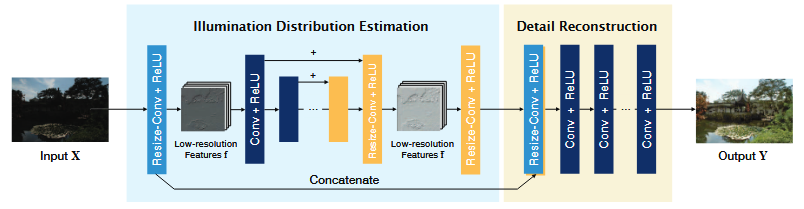
\includegraphics[width=0.8\columnwidth]{GLADNet}
		
		\begin{subfigure}{0.2\textwidth}
			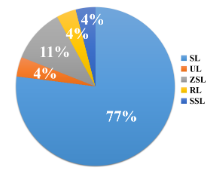
\includegraphics[width=\linewidth]{learning_strategy}
			\captionsetup{font=scriptsize}
			\caption{learning strategy}
			\label{fig:subfig_a}
		\end{subfigure}
		\begin{subfigure}{0.2\textwidth}
			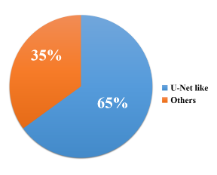
\includegraphics[width=1.15\linewidth]{network_struture}
			\captionsetup{font=scriptsize}
			\caption{network structure}
			\label{fig:subfig_b}
		\end{subfigure}
		\begin{subfigure}{0.2\textwidth}
			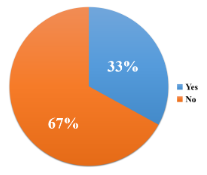
\includegraphics[width=\linewidth]{Retinex_model}
			\captionsetup{font=scriptsize}
			\caption{Retinex model}
			\label{fig:subfig_c}	
		\end{subfigure}
		\begin{subfigure}{0.2\textwidth}
			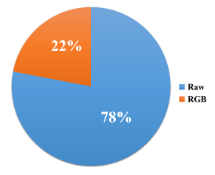
\includegraphics[width=\linewidth]{data_format}
			\captionsetup{font=scriptsize}
			\caption{data format}
			\label{fig:subfig_d}
		\end{subfigure}\\
		\begin{subfigure}{0.2\textwidth}
			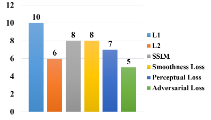
\includegraphics[width=\linewidth]{loss_function}
			\captionsetup{font=scriptsize}
			\caption{loss function}
			\label{fig:subfig_e}
		\end{subfigure}
		\begin{subfigure}{0.2\textwidth}
			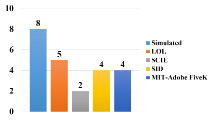
\includegraphics[width=\linewidth]{training_dataset}
			\captionsetup{font=scriptsize}
			\caption{training dataset}
			\label{fig:subfig_f}	
		\end{subfigure}	
		\begin{subfigure}{0.2\textwidth}
			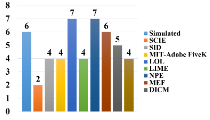
\includegraphics[width=\linewidth]{testing_dataset}
			\captionsetup{font=scriptsize}
			\caption{testing dataset}
			\label{fig:subfig_g}
		\end{subfigure}
		\begin{subfigure}{0.2\textwidth}
			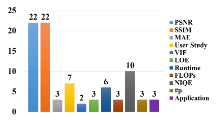
\includegraphics[width=\linewidth]{evaluation_metric}
			\captionsetup{font=scriptsize}
			\caption{evaluation metric}
			\label{fig:subfig_h}	
		\end{subfigure}
		\captionsetup{font=scriptsize}
		\caption{
			\label{fig: Statictic Analysis} % spaces are big no-no withing labels
			% things like fig: are optional in the label but it helps
			% to orient yourself when you have multiple figures,
			% equations and tables
			A statictic analysis of deep learning-based LLIE methods, including learning strategy, network characteristic, Retinex model, data format, loss function, training dataset, testing dataset, and evaluation metric. Better to see with zoom.
		}
	\end{figure}
	
	
	\paragraph{Network Structure} \qquad
	
	从Fig.\ref{fig:subfig_b}可以看来,UNet及类UNet架构占据LLIE的65\%。这是因为:UNet可以有效的集成多尺度特征并同时采用低级与高级特征。这种特性对于取得令人满意的地低光增强非常重要。
	尽管如此,有这样几个问题可能被当前的LLIE网络结构忽略了:
	
	(1) 经过多个卷积层处理后,由于比较小的像素值,极低光图像的梯度可能会在梯度反向传统过程中消失,这可能会导致模型性能并影响网络的收敛;
	
	(2) UNet中的跳过连接可能会引入噪声和冗余特征到最后的结果。如何有效的滤除噪声并同时集成低级与高级特征应该仔细考虑;
	
	(3) 尽管针对LLIE提出了部分设计和成分,但它们往往是从其他相关low-level中修改而来。在设计网络时,低光图像的特征同样应当考虑在内。
	
	
	\paragraph{Combination of Deep Model and Retinex Theory} \qquad
	
	从Fig.\ref{fig:subfig_c}可以看到:近三分之一的方法采用了深度学习+Retinex组合的方式进行设计,采用不同的子网络估计Retinex的不同成分,并估计亮度以引导网络的学习。尽管这种组合可以在深度学习与Retinex之间进行很好的桥接,但可能同时引入各自的弱点到最终的模型:
	
	(1) Retinex的理想假设可能会影响最终的结果;
	
	(2) 深度学习的过拟合可能仍存在;
	
	当组合深度学习与Retinex设计网络时,如何从两者中“取其精华去其糟粕”应该慎重考虑。
	
	
	\paragraph{Data Format} \qquad
	
	正如Fig.\ref{fig:subfig_d}所示,RAW数据是大多数据方法的首选。尽管RAW数据会受限于特定的传感器,但其包含更多的色域以及更高的动态范围。因此,基于RAW数据的深度模型可以重建更清晰的细节、高对比度,具有更好的色彩信息,同时降低了噪声和伪影问题。
	
	尽管如此,由于智能手机的便捷采集性,RGB形式的图像也被不少方法采用并作为输入。在未来的研究中,RAW数据到RGB格式的平滑变化将更有助于LLIE的研究。
	
	
	\paragraph{Loss Function} \qquad
	
	从Fig.\ref{fig:subfig_e}可以看到:LLIE常采用的损失函数为L1, L2, SSIM,感知损失,平滑损失等。除此之外,按照不同的需求,颜色损失、曝光损失、对抗损失同样也得到了应用。
	
	\paragraph{Training Datasets} \qquad
	
	从Fig.\ref{fig:subfig_f}可以看到:不同的成对训练数据被提出并用于LLIE方案的训练。这些数据包含真实数据与合成数据,相关信息见Table \ref{tab: Paired_training_datases}。
	
	\begin{table}[!htbp]
		\centering
		\tiny
		%\resizebox{\textwidth}{!}{ %按照宽度调整调整表格大小
			\begin{tabular}{>{\centering\arraybackslash}m{2.5cm}|c|c|c|c}
				
				\hline
				
				\textbf{Name} & \textbf{Number} & \textbf{Format} & \textbf{Real/Syn} & \textbf{Video} \\
				
				\hline
				
				Gamma Correction & $+\infty$ & RGB & Syn & \\
				
				Random Illumination & $+\infty$ & RGB & Syn & \\
				
				\hline
				
				LOL\cite{wei2018deep} & 500 & RGB & Real & \\
				
				SCIE\cite{cai2018learning} & 4,413 & RGB & Real & \\
				
				VE-LOL-L\cite{jiang2019learning} & 2,500 & RGB & Real+Syn & \\
				
				MIT-Adobe FiveK\cite{bychkovsky2011learning} & 5,000 & Raw & Real & \\
				
				SID\cite{wei2018deep} & 5,094 & Raw & Real & \\
				
				DRV\cite{chen2019seeing} & 202 & Raw & Real & \checkmark  \\
				
				SMOID\cite{jiang2019learning} & 179 & Raw & Real & \checkmark  \\
				
				\hline
				
			\end{tabular}
			%}
		\captionsetup{font=scriptsize} %设置标题字体与表格字体一致
		\caption{\label{tab: Paired_training_datases}
			Summary of paired training datasets. 'Syn' represents Synthetic.} %表格的标题
		
	\end{table}
	
	\paragraph{Testing Dataset} \qquad
	
	除了上述训练数据集外,还有一些测试数据集,相关信息如Table \ref{tab: Testing datasets}所示。
	
		\begin{table}[!htbp]
		\centering
		\tiny
		%\resizebox{\textwidth}{!}{ %按照宽度调整调整表格大小
			\begin{tabular}{>{\centering\arraybackslash}m{2.5cm}|c|c|c|c}
				
				\hline
				
				\textbf{Name} & \textbf{Number} & \textbf{Format} & \textbf{Application} & \textbf{Video} \\
				
				\hline
				
				LIME\cite{guo2016lime} & 10 & RGB & &  \\ 
				NPE\cite{wang2013naturalness}  & 84 & RGB & &  \\ 
				MEF\cite{lee2011power}  & 17 & RGB & &  \\
				DICM\cite{lee2013contrast} & 64 & RGB & &  \\
			 $\text{VV}^{2}$& 24 & RGB & &  \\
			 
			 	\hline
			 	
				BBD-100K\cite{yu2020bdd100k} & 10,000 & RGB & \checkmark & \checkmark \\
				ExDARK\cite{loh2019getting} & 7,363 & RGB & \checkmark & \\ 
				DARK FACE\cite{yuan2019ug} & 6,000 & RGB & \checkmark & \\
				VE-LOL-H\cite{jiang2019learning} & 10,940 & RGB & \checkmark & \\
				
				\hline
				
			\end{tabular}
			%}
		\captionsetup{font=scriptsize} %设置标题字体与表格字体一致
		\caption{\label{tab: Testing datasets}
			Summary of testing datasets.} %表格的标题
		
		\end{table}
	
	\paragraph{Benchmarking and Empirical Analysis} \qquad
	
	在这部分内容中,我们将对现有基于深度学习的LLIE方法进行分析并突出存在的关键挑战。为方便分析,我们提出了一个大尺度低光图像/视频数据以验证不同深度学习方法的性能。除此之外,我们开发了首个在线平台,它包含多种深度学习LLIE方法,用户能够以更友好的交互方式重建不同方法的效果。作者对比的方法有13种,它们分别是:
	
	(1) 监督学习方案:LLNet、LightenNet、Retinex-Net、MBLLEN、KinD、KinD++、TBEFN、DSLR;
	
	(2) 无监督方案:EnlightenGAN;
	
	(3)	半监督方案:DRBN;
	
	(4)	Zero-shot方案:ExCNet、Zero-DCE、RRDNet。
	
	
	\paragraph{A New Low-light Image and Video Dataset} \qquad
	
	作者提出一个大尺度低光图像/视频数据集LoLi-Phone,以进行不同LLIE方案系统而详细的验证对比。LoLi-Phone是目前为止最大的真实低光图像数据。数据与采集设备信息见Table \ref{tab: LoLi-Phone dataset}与Figure 4。
	
		\begin{table}[!htbp]
		\centering
		\tiny
		%\resizebox{\textwidth}{!}{ %按照宽度调整调整表格大小
			\begin{tabular}{>{\centering\arraybackslash}m{2.5cm}|c|c|c}
				
				\hline
				
				\textbf{Phone's Brand} & \textbf{\#Video} & \textbf{\#Image} & \textbf{Resolution} \\
				
				\hline
				
				iPhone 6s   		& 4 & 1,029	& 1920×1080 \\
				iPhone 7 	 		& 13& 6,081 & 1920×1080 \\
				iPhone7 Plus		& 2 & 900   & 1920×1080 \\
				iPhone8 Plus 		& 1 & 489   & 1280×720  \\
				iPhone 11   		& 7 & 2,200 & 1920×1080 \\
				iPhone 11 Pro 		& 17& 7,739 & 1920×1080 \\
				iPhone XS 	 		& 11& 2,470 & 1920×1080 \\
				iPhone XR 			& 16& 4,997 & 1920×1080 \\
				iPhone SE 			& 1 & 455   & 1920×1080 \\
				Xiaomi Mi 9	 		& 2 & 1,145 & 1920×1080 \\
				Xiaomi Mi Mix 3     & 6 & 2,972 & 1920×1080 \\
				Pixel 3   			& 4 & 1,311 & 1920×1080 \\
				Pixel 4   			& 3 & 1,1923& 1920×1080 \\
				Oppo R17 			& 6 & 2,126 & 1920×1080 \\
				Vivo Nex 	 		& 12& 4,097 & 1280×720  \\
				LG M322      		& 2 & 761   & 1920×1080 \\
				OnePlus 5T   		& 1 & 293   & 1920×1080 \\
				Huawei Mate 20 Pro 	& 12& 4,160 & 1920×1080 \\
				
				\hline
				
			\end{tabular}
			%}
		\captionsetup{font=scriptsize} %设置标题字体与表格字体一致
		\caption{\label{tab: LoLi-Phone dataset}
			Summary of LoLi-Phone dataset. LoLi-Phone dataset contains 120 videos (55,148 images) taken by 18 different mobile phones' cameras. "\#Video" and "\#Image" represent the number of videos and images, respectively.} %表格的标题
		
	\end{table}
	
	\begin{figure}[ht] 
		% read manual to see what [ht] means and for other possible options
		\centering 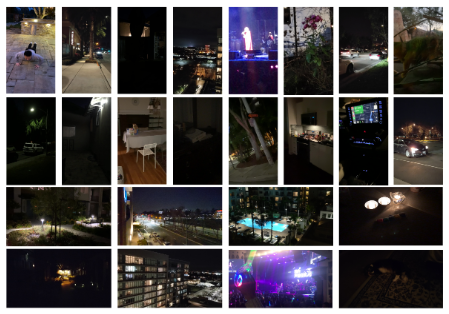
\includegraphics[width=0.8\columnwidth]{Sample_Loli}
		\caption{
			\label{fig:Sample_Loli} % spaces are big no-no withing labels
			% things like fig: are optional in the label but it helps
			% to orient yourself when you have multiple figures,
			% equations and tables
			Several images sampled from the proposed LoLiPhone dataset. The images and videos are taken by different devices under diverse lighting conditions and scenes.
		}
	\end{figure}
	
	\paragraph{Online Evaluation Platform} \qquad
	
	不同方法可能采用不同的深度学习框架,比如Caffe、Theano、TensorFlow以及Pytorch,因此,不同的方法依赖于不同的配置、GPU版本以及硬件信息。这样复杂的需求对于研究员极度不友好,尤其对于出入门者,甚至没有GPU资源的研究员。为缓解该问题,我们开发了在线LLIE平台,称之为LoLi-Platform\footnote{http://mc.nankai.edu.cn/ll/}。
	
	\paragraph{Benchmark Results} \qquad
	
	为更好的定量与定性对比不同的方法,除了LoLi-Phone外,作者还在LOL与MIT-Adboe FiveK数据集上进行了对比。
	
	\begin{figure}[htbp] 
		\centering 
		\begin{subfigure}{0.18\textwidth}
			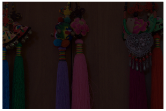
\includegraphics[width=\linewidth]{LOL-test_dataset/input}
			\captionsetup{font=scriptsize}
			\caption{input}
			\label{fig: LOL-test_a}
		\end{subfigure}
		\begin{subfigure}{0.18\textwidth}
			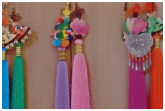
\includegraphics[width=\linewidth]{LOL-test_dataset/LLNet}
			\captionsetup{font=scriptsize}
			\caption{LLNet}
			\label{fig: LOL-test_b}
		\end{subfigure}
		\begin{subfigure}{0.18\textwidth}
			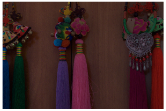
\includegraphics[width=\linewidth]{LOL-test_dataset/LightenNet}
			\captionsetup{font=scriptsize}
			\caption{LightenNet}
			\label{fig: LOL-test_c}  
		\end{subfigure}
		\begin{subfigure}{0.18\textwidth}
			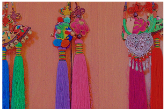
\includegraphics[width=\linewidth]{LOL-test_dataset/Retinex-Net}
			\captionsetup{font=scriptsize}
			\caption{Retinex-Net}
			\label{fig: LOL-test_d}
		\end{subfigure}
		\begin{subfigure}{0.18\textwidth}
			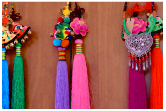
\includegraphics[width=\linewidth]{LOL-test_dataset/MBLLEN}
			\captionsetup{font=scriptsize}
			\caption{MBLLEN}
			\label{fig: LOL-test_e}
		\end{subfigure}\\
		\begin{subfigure}{0.18\textwidth}
			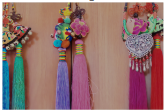
\includegraphics[width=\linewidth]{LOL-test_dataset/KinD}
			\captionsetup{font=scriptsize}
			\caption{KinD}
			\label{fig: LOL-test_f}  
		\end{subfigure}    
		\begin{subfigure}{0.18\textwidth}
			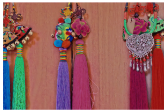
\includegraphics[width=\linewidth]{LOL-test_dataset/KinD++}
			\captionsetup{font=scriptsize}
			\caption{KinD++}
			\label{fig: LOL-test_g}
		\end{subfigure}
		\begin{subfigure}{0.18\textwidth}
			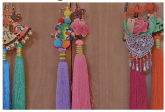
\includegraphics[width=\linewidth]{LOL-test_dataset/TBEFN}
			\captionsetup{font=scriptsize}
			\caption{TBEFN}
			\label{fig: LOL-test_h}  
		\end{subfigure}
		\begin{subfigure}{0.18\textwidth}
			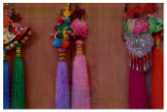
\includegraphics[width=\linewidth]{LOL-test_dataset/DSLR}
			\captionsetup{font=scriptsize}
			\caption{DSLR}
			\label{fig: LOL-test_i}  
		\end{subfigure}
		\begin{subfigure}{0.18\textwidth}
			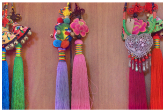
\includegraphics[width=\linewidth]{LOL-test_dataset/EnlightenGAN}
			\captionsetup{font=scriptsize}
			\caption{EnlightenGAN}
			\label{fig: LOL-test_j}  
		\end{subfigure}\\
		\begin{subfigure}{0.18\textwidth}
			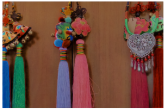
\includegraphics[width=\linewidth]{LOL-test_dataset/DRBN}
			\captionsetup{font=scriptsize}
			\caption{DRBN}
			\label{fig: LOL-test_k}  
		\end{subfigure}    
		\begin{subfigure}{0.18\textwidth}
			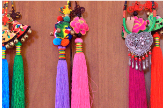
\includegraphics[width=\linewidth]{LOL-test_dataset/ExCNet}
			\captionsetup{font=scriptsize}
			\caption{ExCNet}
			\label{fig: LOL-test_l}
		\end{subfigure}
		\begin{subfigure}{0.18\textwidth}
			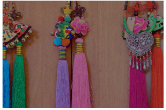
\includegraphics[width=\linewidth]{LOL-test_dataset/Zero-DCE}
			\captionsetup{font=scriptsize}
			\caption{Zero-DCE}
			\label{fig: LOL-test_m}  
		\end{subfigure}
		\begin{subfigure}{0.18\textwidth}
			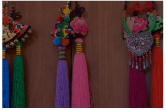
\includegraphics[width=\linewidth]{LOL-test_dataset/RRDNet}
			\captionsetup{font=scriptsize}
			\caption{RRDNet}
			\label{fig: LOL-test_n}  
		\end{subfigure}
		\begin{subfigure}{0.18\textwidth}
			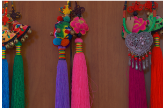
\includegraphics[width=\linewidth]{LOL-test_dataset/GT}
			\captionsetup{font=scriptsize}
			\caption{GT}
			\label{fig: LOL-test_o}  
		\end{subfigure}
		
		\captionsetup{font=scriptsize}
		\caption{
			\label{fig: Visual Result from LOL-test dataset}
			Visual results of different methods on a low-light image sampled from LOL-test dataset.
		}
	\end{figure}
	
	\begin{figure}[htbp] 
		\centering 
		\begin{subfigure}{0.18\textwidth}
			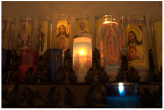
\includegraphics[width=\linewidth]{MIT-Adobe_FiveK/input}
			\captionsetup{font=scriptsize}
			\caption{input}
			\label{fig: MIT-Adobe_FiveK_a}
		\end{subfigure}
		\begin{subfigure}{0.18\textwidth}
			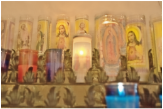
\includegraphics[width=\linewidth]{MIT-Adobe_FiveK/LLNet}
			\captionsetup{font=scriptsize}
			\caption{LLNet}
			\label{fig: MIT-Adobe_FiveK_b}
		\end{subfigure}
		\begin{subfigure}{0.18\textwidth}
			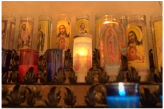
\includegraphics[width=\linewidth]{MIT-Adobe_FiveK/LightenNet}
			\captionsetup{font=scriptsize}
			\caption{LightenNet}
			\label{fig: MIT-Adobe_FiveK_c}  
		\end{subfigure}
		\begin{subfigure}{0.18\textwidth}
			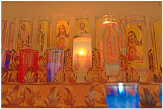
\includegraphics[width=\linewidth]{MIT-Adobe_FiveK/Retinex-Net}
			\captionsetup{font=scriptsize}
			\caption{Retinex-Net}
			\label{fig: MIT-Adobe_FiveK_d}
		\end{subfigure}
		\begin{subfigure}{0.18\textwidth}
			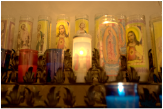
\includegraphics[width=\linewidth]{MIT-Adobe_FiveK/MBLLEN}
			\captionsetup{font=scriptsize}
			\caption{MBLLEN}
			\label{fig: MIT-Adobe_FiveK_e}
		\end{subfigure}\\
		\begin{subfigure}{0.18\textwidth}
			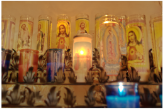
\includegraphics[width=\linewidth]{MIT-Adobe_FiveK/KinD}
			\captionsetup{font=scriptsize}
			\caption{KinD}
			\label{fig: MIT-Adobe_FiveK_f}  
		\end{subfigure}    
		\begin{subfigure}{0.18\textwidth}
			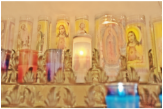
\includegraphics[width=\linewidth]{MIT-Adobe_FiveK/KinD++}
			\captionsetup{font=scriptsize}
			\caption{KinD++}
			\label{fig: MIT-Adobe_FiveK_g}
		\end{subfigure}
		\begin{subfigure}{0.18\textwidth}
			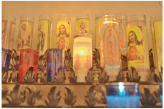
\includegraphics[width=\linewidth]{MIT-Adobe_FiveK/TBEFN}
			\captionsetup{font=scriptsize}
			\caption{TBEFN}
			\label{fig: MIT-Adobe_FiveK_h}  
		\end{subfigure}
		\begin{subfigure}{0.18\textwidth}
			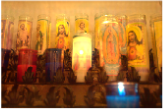
\includegraphics[width=\linewidth]{MIT-Adobe_FiveK/DSLR}
			\captionsetup{font=scriptsize}
			\caption{DSLR}
			\label{fig: MIT-Adobe_FiveK_i}  
		\end{subfigure}
		\begin{subfigure}{0.18\textwidth}
			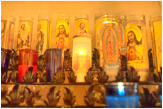
\includegraphics[width=\linewidth]{MIT-Adobe_FiveK/EnlightenGAN}
			\captionsetup{font=scriptsize}
			\caption{EnlightenGAN}
			\label{fig: MIT-Adobe_FiveK_j}  
		\end{subfigure}\\
		\begin{subfigure}{0.18\textwidth}
			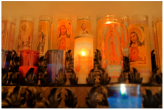
\includegraphics[width=\linewidth]{MIT-Adobe_FiveK/DRBN}
			\captionsetup{font=scriptsize}
			\caption{DRBN}
			\label{fig: MIT-Adobe_FiveK_k}  
		\end{subfigure}    
		\begin{subfigure}{0.18\textwidth}
			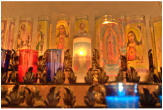
\includegraphics[width=\linewidth]{MIT-Adobe_FiveK/ExCNet}
			\captionsetup{font=scriptsize}
			\caption{ExCNet}
			\label{fig: MIT-Adobe_FiveK_l}
		\end{subfigure}
		\begin{subfigure}{0.18\textwidth}
			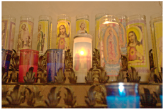
\includegraphics[width=\linewidth]{MIT-Adobe_FiveK/Zero-DCE}
			\captionsetup{font=scriptsize}
			\caption{Zero-DCE}
			\label{fig: MIT-Adobe_FiveK_m}  
		\end{subfigure}
		\begin{subfigure}{0.18\textwidth}
			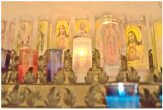
\includegraphics[width=\linewidth]{MIT-Adobe_FiveK/RRDNet}
			\captionsetup{font=scriptsize}
			\caption{RRDNet}
			\label{fig: MIT-Adobe_FiveK_n}  
		\end{subfigure}
		\begin{subfigure}{0.18\textwidth}
			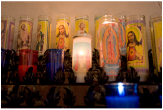
\includegraphics[width=\linewidth]{MIT-Adobe_FiveK/GT}
			\captionsetup{font=scriptsize}
			\caption{GT}
			\label{fig: MIT-Adobe_FiveK_o}  
		\end{subfigure}
		
		\captionsetup{font=scriptsize}
		\caption{
			\label{fig: Visual Result from MIT-Adobe FiveK dataset}
			Visual results of different methods on a low-light image sampled from MIT-Adobe FiveK-test dataset.
		}
	\end{figure}
	
	Fig.\ref{fig: Visual Result from LOL-test dataset}和Fig.\ref{fig: Visual Result from MIT-Adobe FiveK dataset}对比了不同方法在LOL与FiveK数据上的效果对比,可以看到:
	
	在LOL测试数据集上有以下几点发现:
	
	(1) 所有方法均提升了输入图像的亮度和对比,但没有一个能成功进行色彩重建;
	
	(2) LLNet产生了比较的结果;
	
	(3) LightenNet、RRDNet生成欠曝结果,而MBLLEN、ExCNet则生成过曝结果;
	
	(4) KinD、KinD++、TBEFN、DSLR、EnlightenGAN、DRBN则引入明显的伪影;
	
	在FiveK数据集上有以下几点发现:
	
	(1) LLNet、KinD++、TBEFN、RRDNet生成了过曝结果;
	
	(2) Retinex-Net、KinD++、RRDNet生成了伪影,同时又模糊问题。
	
	\begin{figure}[htbp] 
		\centering 
		\begin{subfigure}{0.128\textwidth}
			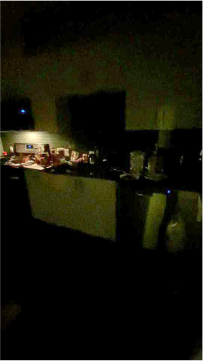
\includegraphics[width=\linewidth]{LoLi-Phone-imgT/input}
			\captionsetup{font=scriptsize}
			\caption{}
			\label{fig: LoLi-Phone-imgT_a}
		\end{subfigure}
		\begin{subfigure}{0.128\textwidth}
			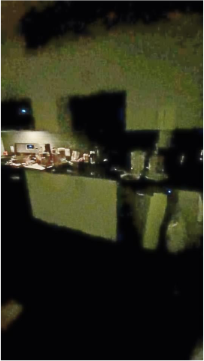
\includegraphics[width=\linewidth]{LoLi-Phone-imgT/LLNet}
			\captionsetup{font=scriptsize}
			\caption{}
			\label{fig: LoLi-Phone-imgT_b}
		\end{subfigure}
		\begin{subfigure}{0.128\textwidth}
			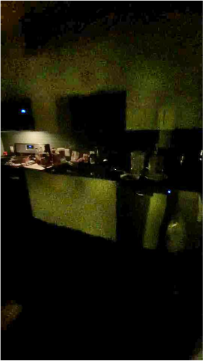
\includegraphics[width=\linewidth]{LoLi-Phone-imgT/LightenNet}
			\captionsetup{font=scriptsize}
			\caption{}
			\label{fig: LoLi-Phone-imgT_c}  
		\end{subfigure}
		\begin{subfigure}{0.128\textwidth}
			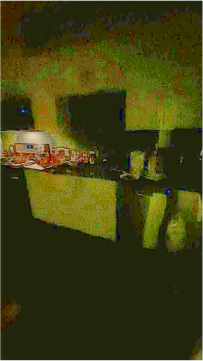
\includegraphics[width=\linewidth]{LoLi-Phone-imgT/Retinex-Net}
			\captionsetup{font=scriptsize}
			\caption{}
			\label{fig: LoLi-Phone-imgT_d}
		\end{subfigure}
		\begin{subfigure}{0.128\textwidth}
			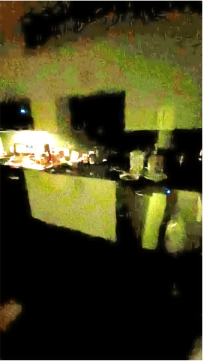
\includegraphics[width=\linewidth]{LoLi-Phone-imgT/MBLLEN}
			\captionsetup{font=scriptsize}
			\caption{}
			\label{fig: LoLi-Phone-imgT_e}
		\end{subfigure}
		\begin{subfigure}{0.128\textwidth}
			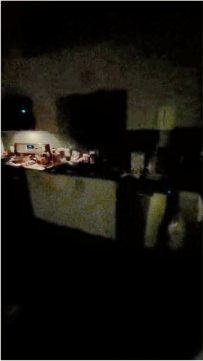
\includegraphics[width=\linewidth]{LoLi-Phone-imgT/KinD}
			\captionsetup{font=scriptsize}
			\caption{}
			\label{fig: LoLi-Phone-imgT_f}  
		\end{subfigure}    
		\begin{subfigure}{0.128\textwidth}
			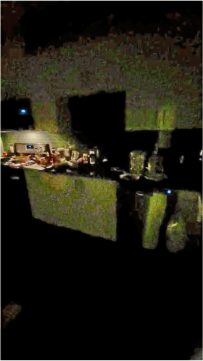
\includegraphics[width=\linewidth]{LoLi-Phone-imgT/KinD++}
			\captionsetup{font=scriptsize}
			\caption{}
			\label{fig: LoLi-Phone-imgT_g}
		\end{subfigure}\\
		\begin{subfigure}{0.128\textwidth}
			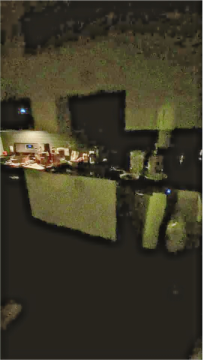
\includegraphics[width=\linewidth]{LoLi-Phone-imgT/TBEFN}
			\captionsetup{font=scriptsize}
			\caption{}
			\label{fig: LoLi-Phone-imgT_h}  
		\end{subfigure}
		\begin{subfigure}{0.128\textwidth}
			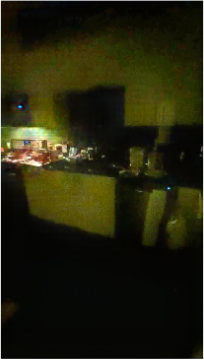
\includegraphics[width=\linewidth]{LoLi-Phone-imgT/DSLR}
			\captionsetup{font=scriptsize}
			\caption{}
			\label{fig: LoLi-Phone-imgT_i}  
		\end{subfigure}
		\begin{subfigure}{0.128\textwidth}
			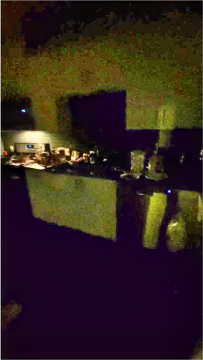
\includegraphics[width=\linewidth]{LoLi-Phone-imgT/EnlightenGAN}
			\captionsetup{font=scriptsize}
			\caption{}
			\label{fig: LoLi-Phone-imgT_j}  
		\end{subfigure}
		\begin{subfigure}{0.128\textwidth}
			\includegraphics[width=\linewidth]{LoLi-Phone-imgT/DRBN}
			\captionsetup{font=scriptsize}
			\caption{}
			\label{fig: LoLi-Phone-imgT_k}  
		\end{subfigure}    
		\begin{subfigure}{0.128\textwidth}
			\includegraphics[width=\linewidth]{LoLi-Phone-imgT/ExCNet}
			\captionsetup{font=scriptsize}
			\caption{}
			\label{fig: LoLi-Phone-imgT_l}
		\end{subfigure}
		\begin{subfigure}{0.128\textwidth}
			\includegraphics[width=\linewidth]{LoLi-Phone-imgT/Zero-DCE}
			\captionsetup{font=scriptsize}
			\caption{}
			\label{fig: LoLi-Phone-imgT_m}  
		\end{subfigure}
		\begin{subfigure}{0.128\textwidth}
			\includegraphics[width=\linewidth]{LoLi-Phone-imgT/RRDNet}
			\captionsetup{font=scriptsize}
			\caption{}
			\label{fig: LoLi-Phone-imgT_n}  
		\end{subfigure}\\
		
		\captionsetup{font=scriptsize}
		\caption{
			\label{fig: Visual Result from LoLi-Phone-imgT dataset}
			Visual results of different methods on a low-light image sampled from LoLi-Phone-imgT dataset. (a) input (b) LLNet (c) LightenNet (d) Retinex-Net (e) MBLLEN  (f) KinD  (g) KinD++  (h) TBEFN  (i) DSLR  (j) EnlightenGAN  (k) DRBN  (l) ExCNet  (m) Zero-DCE  (n) RRDNet 
		}
	\end{figure}
	
	
	\begin{figure}[htbp] 
		\centering 
		\begin{subfigure}{0.128\textwidth}
			\includegraphics[width=\linewidth]{LoLi-Phone-imgT_1/input}
			\captionsetup{font=scriptsize}
			\caption{}
			\label{fig: LoLi-Phone-imgT_1_a}
		\end{subfigure}
		\begin{subfigure}{0.128\textwidth}
			\includegraphics[width=\linewidth]{LoLi-Phone-imgT_1/LLNet}
			\captionsetup{font=scriptsize}
			\caption{}
			\label{fig: LoLi-Phone-imgT_1_b}
		\end{subfigure}
		\begin{subfigure}{0.128\textwidth}
			\includegraphics[width=\linewidth]{LoLi-Phone-imgT_1/LightenNet}
			\captionsetup{font=scriptsize}
			\caption{}
			\label{fig: LoLi-Phone-imgT_1_c}  
		\end{subfigure}
		\begin{subfigure}{0.128\textwidth}
			\includegraphics[width=\linewidth]{LoLi-Phone-imgT_1/Retinex-Net}
			\captionsetup{font=scriptsize}
			\caption{}
			\label{fig: LoLi-Phone-imgT_1_d}
		\end{subfigure}
		\begin{subfigure}{0.128\textwidth}
			\includegraphics[width=\linewidth]{LoLi-Phone-imgT_1/MBLLEN}
			\captionsetup{font=scriptsize}
			\caption{}
			\label{fig: LoLi-Phone-imgT_1_e}
		\end{subfigure}
		\begin{subfigure}{0.128\textwidth}
			\includegraphics[width=\linewidth]{LoLi-Phone-imgT_1/KinD}
			\captionsetup{font=scriptsize}
			\caption{}
			\label{fig: LoLi-Phone-imgT_1_f}  
		\end{subfigure}    
		\begin{subfigure}{0.128\textwidth}
			\includegraphics[width=\linewidth]{LoLi-Phone-imgT_1/KinD++}
			\captionsetup{font=scriptsize}
			\caption{}
			\label{fig: LoLi-Phone-imgT_1_g}
		\end{subfigure}\\
		\begin{subfigure}{0.128\textwidth}
			\includegraphics[width=\linewidth]{LoLi-Phone-imgT_1/TBEFN}
			\captionsetup{font=scriptsize}
			\caption{}
			\label{fig: LoLi-Phone-imgT_1_h}  
		\end{subfigure}
		\begin{subfigure}{0.128\textwidth}
			\includegraphics[width=\linewidth]{LoLi-Phone-imgT_1/DSLR}
			\captionsetup{font=scriptsize}
			\caption{}
			\label{fig: LoLi-Phone-imgT_1_i}  
		\end{subfigure}
		\begin{subfigure}{0.128\textwidth}
			\includegraphics[width=\linewidth]{LoLi-Phone-imgT_1/EnlightenGAN}
			\captionsetup{font=scriptsize}
			\caption{}
			\label{fig: LoLi-Phone-imgT_1_j}  
		\end{subfigure}
		\begin{subfigure}{0.128\textwidth}
			\includegraphics[width=\linewidth]{LoLi-Phone-imgT_1/DRBN}
			\captionsetup{font=scriptsize}
			\caption{}
			\label{fig: LoLi-Phone-imgT_1_k}  
		\end{subfigure}    
		\begin{subfigure}{0.128\textwidth}
			\includegraphics[width=\linewidth]{LoLi-Phone-imgT_1/ExCNet}
			\captionsetup{font=scriptsize}
			\caption{}
			\label{fig: LoLi-Phone-imgT_1_l}
		\end{subfigure}
		\begin{subfigure}{0.128\textwidth}
			\includegraphics[width=\linewidth]{LoLi-Phone-imgT_1/Zero-DCE}
			\captionsetup{font=scriptsize}
			\caption{}
			\label{fig: LoLi-Phone-imgT_1_m}  
		\end{subfigure}
		\begin{subfigure}{0.128\textwidth}
			\includegraphics[width=\linewidth]{LoLi-Phone-imgT_1/RRDNet}
			\captionsetup{font=scriptsize}
			\caption{}
			\label{fig: LoLi-Phone-imgT_1_n}  
		\end{subfigure}\\
		
		\captionsetup{font=scriptsize}
		\caption{
			\label{fig: Visual Result from LoLi-Phone-imgT_1 dataset}
			Visual results of different methods on a low-light image sampled from LoLi-Phone-imgT dataset. (a) input (b) LLNet (c) LightenNet (d) Retinex-Net (e) MBLLEN  (f) KinD  (g) KinD++  (h) TBEFN  (i) DSLR  (j) EnlightenGAN  (k) DRBN  (l) ExCNet  (m) Zero-DCE  (n) RRDNet 
		}
	\end{figure}
	
	Fig.\ref{fig: Visual Result from LoLi-Phone-imgT dataset} 和Fig.\ref{fig: Visual Result from LoLi-Phone-imgT_1 dataset}给出了LoLi-Phone数据集上的效果对比,可以看到:
	
	对于Fig.\ref{fig: Visual Result from LoLi-Phone-imgT dataset}有以下几点发现:
	
	(1) 所有方法均无法有效改进亮度并移除噪声;
	
	(2) Retinex-Net、MBLLEN、DRBN生成了明显伪影;
	
	对于和Fig.\ref{fig: Visual Result from LoLi-Phone-imgT_1 dataset}有以下几点发现:
	
	(1) 所有方法均增强了输入图像的亮度;
	
	(2) 仅有MBLLEN、RRDNet取得视觉友好的增强效果,且无色片、伪影以及欠/过曝问题。
	
	
	\begin{table}[!htbp]
		\centering
		\tiny
		\resizebox{\textwidth}{!}{ %按照宽度调整调整表格大小
			\begin{tabular}{>{\centering\arraybackslash}m{2cm}|>{\centering\arraybackslash}m{2.5cm}|c|c|c|c|c|c|c|c}
				
				\hline %添加表格头部粗线
				
				% \multirow{2}*{\textbf{Learning}} & \multirow{2}*{\textbf{Mathod}} & \multicolumn{4}{c|}{\textbf{LOL-test}} & \multicolumn{4}{c}{\textbf{MIT-Adobe FiveK-test}} \\
				
				\multirowcell{2}{\centering\textbf{Learning}} & \multirowcell{2}{\textbf{Method}} & \multicolumn{4}{c|}{\makecell{\textbf{LOL-test}}} & \multicolumn{4}{c}{\makecell{\textbf{MIT-Adobe FiveK-test}}} \\
				
				\cline{3-10}
				
				
				& 		 & \textbf{MSE↓}  & \textbf{PSNR↑} & \textbf{SSIM↑} & \textbf{LPIPS↓} & \textbf{MSE↓}  & \textbf{PSNR↑}  & \textbf{SSIM↑} & \textbf{LPIPS↓} \\
				
				\hline
				
				& input & 12.613& 7.773 & 0.181 & 0.560  & 1.670 & 17.824 & 0.779 & 0.148  \\
				
				\hline	
				
				\multirowcell{8}{SL} & LLNet & 1.290 & 17.959& 0.713 & 0.360  & 4.465 & 12.177 & 0.645 & 0.292 \\
				& LightenNet & 7.614 & 10.301& 0.402 & 0.394  & 4.127 & 13.579 & 0.744 & 0.166 \\
				& Retinex-Net& 1.651 & 16.774& 0.462 & 0.474  & 4.406 & 12.310 & 0.671 & 0.239 \\
				& MBLLEN 	 & 1.444 & 17.902& 0.715 & 0.247  &	1.296 & 19.781 & 0.825 & 0.108 \\
				& KinD 		 & 1.431 & 17.648& 0.779 & 0.175  & 2.675 & 14.535 & 0.741 & 0.177 \\
				& KinD++     & 1.298 & 17.752& 0.760 & 0.198  & 7.582 & 9.732  & 0.568 & 0.336 \\
				& TBEFN 	 & 1.764 & 17.351& 0.786 & 0.210  & 3.865 & 12.769 & 0.704 & 0.178 \\
				& DSLR 		 & 3.536 & 15.050& 0.597 & 0.337  & 1.925 & 16.632 & 0.782 & 0.167 \\
				
				\hline
				
				UL & EnlightenGAN & 1.998 & 17.483& 0.677 & 0.322  & 3.628 & 13.260 & 0.745 & 0.170 \\
				
				\hline
				
				SSL  & DRBN       & 2.359 & 15.125& 0.472 & 0.316  & 3.314 & 13.355 & 0.378 & 0.281 \\ 
				
				\hline
				
				\multirowcell{3}{ZSL} & ExCNet&2.292 & 15.783& 0.515 & 0.373  & 2.927 & 13.978 & 0.710 0.187   \\
				& Zero-DCE 	 & 3.282 & 14.861& 0.589 & 0.335  & 3.476 & 13.199 & 0.709 0.203   \\
				& RRDNet     & 6.313 & 11.392& 0.468 & 0.361  & 7.057 & 10.135 & 0.620 0.303   \\
				
				
				\hline
				
			\end{tabular}
		}
		\captionsetup{font=scriptsize} %设置标题字体与表格字体一致
		\caption{\label{tab: Quantitative Comparisons on LOL-test and MIT-Adobe FiveK-test testing datasets}
			Quantitative comparisons on LOL-test and MIT-Adobe FiveK-test testing datasets in terms of MSE (×103), PSNR (in dB), SSIM, and LPIPS. The best result is in red whereas the second and third best results are in blue and purple under each case, respectively.} %表格的标题
		
	\end{table}
	
	\begin{table}[!htbp]
		\centering
		\tiny
		% \resizebox{\textwidth}{!}{ %按照宽度调整调整表格大小
			\begin{tabular}{>{\centering\arraybackslash}m{2cm}|>{\centering\arraybackslash}m{2.5cm}|c|c|c|c}
				
				\hline %添加表格头部粗线
				
				% \multirow{2}*{\textbf{Learning}} & \multirow{2}*{\textbf{Mathod}} & \multicolumn{4}{c|}{\textbf{LOL-test}} & \multicolumn{4}{c}{\textbf{MIT-Adobe FiveK-test}} \\
				
				\multirowcell{2}{\centering\textbf{Learning}} & \multirowcell{2}{\textbf{Method}} & \multicolumn{4}{c}{\makecell{\textbf{LoLi-Phone-imgT}}}  \\
				
				\cline{3-6}
				
				
				& 		 & \textbf{NIQE↓}  & \textbf{LOE↓} & \textbf{PI↓} & \textbf{SPAQ↑} \\
				
				\hline
				
				& input & 6.99 & \textcolor{red}{0.00} & 5.86 & 44.45 \\
				
				\hline	
				
				\multirowcell{8}{SL} & LLNet & 5.86  & \textcolor{blue}{5.86}   & 5.66 & 40.56   \\
				& LightenNet & 5.34  & 952.33 & 4.58 & 45.74   \\
				& Retinex-Net& 5.01  & 790.21 & \textcolor{red}{3.48} & \textcolor{red}{50.95}   \\
				& MBLLEN 	 & 5.08  & 220.63 & 4.27 & 42.50   \\
				& KinD 		 & 4.97  & 405.88 & 4.37 & 44.79   \\
				& KinD++     & \textcolor{red}{4.73}  & 681.97 & \textcolor{blue}{3.99} & \textcolor{blue}{46.89}   \\
				& TBEFN 	 & 4.81  & 552.91 & 4.30 & 44.14   \\
				& DSLR 		 & \textcolor{blue}{4.77}  & 447.98 & 4.31 & 41.08   \\
				
				\hline
				
				UL & EnlightenGAN & \textcolor{red}{4.79}  & 821.87 & \textcolor{red}{4.19} & 45.48   \\
				
				\hline
				
				SSL  & DRBN       & 5.80  & 885.75 & 5.54 & 42.74   \\ 
				
				\hline
				
				\multirowcell{3}{ZSL}& ExCNet& 5.55 & 723.56 & 4.38 & 46.74   \\
				& Zero-DCE& 5.82 & 307.09 & 4.76 & \textcolor{red}{46.85}   \\
				& RRDNet  & 5.97 & \textcolor{red}{142.89} & 4.84 & 45.31   \\
				
				
				\hline
				
			\end{tabular}
			% }
		\captionsetup{font=scriptsize} %设置标题字体与表格字体一致
		\caption{\label{tab: Quantitative comparisons on LoLi-Phone-imgT dataset}
			Quantitative comparisons on LoLi-Phone-imgT dataset in terms of NIQE, LOE, PI, and SPAQ. The best result is in red whereas the second and third best results are in blue and purple under each case, respectively.} %表格的标题
		
	\end{table}
	
	Table \ref{tab: Quantitative Comparisons on LOL-test and MIT-Adobe FiveK-test testing datasets}给出了不同方法在LOL与FiveK数据上的定量指标对比,可以看到:
	
	
	(1) 有监督方案具有更高的指标;
	
	(2) LLNet在LOL-test数据上取得了最佳MSE与PSNR;
	
	(3) TBEFN在LOL-test数据上取得了最佳SSIM指标;
	
	(4) KinD在LOL-test数据上取得了最佳LPIPS指标;	
	
	(5)对于FiveK-test数据,MBLLEN取得了全面性的指标优先。
	
	
	Table \ref{tab: Quantitative comparisons on LoLi-Phone-imgT dataset}对比了不同方法在LoLi-Phone-imgT数据上的指标对比,可以看到:
	
	(1) Retinex-Net、KinD++、EnlightenGAN具有相对更佳的性能;
	
	(2) Retinex-Net取得了最佳PI与SPAQ指标,然而从视觉效果上看,它仍存在伪影和色偏问题;
	
	(3) KinD++取得了最佳NIQE指标。
	
	\paragraph{Computational Complexity} \qquad
	
	\begin{table}[!htbp]
		\centering
		\tiny
		% \resizebox{\textwidth}{!}{ %按照宽度调整调整表格大小
			\begin{tabular}{>{\centering\arraybackslash}m{1.5cm}|>{\centering\arraybackslash}m{2.5cm}|c|c|c|c}
				
				\hline %添加表格头部粗线
				
				% \multirow{2}*{\textbf{Learning}} & \multirow{2}*{\textbf{Mathod}} & \multicolumn{4}{c|}{\textbf{LOL-test}} & \multicolumn{4}{c}{\textbf{MIT-Adobe FiveK-test}} \\
				
				\textbf{Learning} & \textbf{Method} & \textbf{RunTime↓} & \textbf{\#Parameters↓} & \textbf{FLOPs↓} & \textbf{Platform} \\
				
				\hline	
				
				\multirowcell{8}{SL} & LLNet & 36.270 & 17.908 & 4124.177 & Theano   \\
				& LightenNet & - & \textcolor{red}{0.030} & \textcolor{red}{30.540} & MATLAB   \\
				& Retinex-Net& 0.120 & 0.555 & 587.470 & TensorFlow  \\
				& MBLLEN 	 & 13.995 & \textcolor{purple}{0.450} & 301.120 & TensorFlow   \\
				& KinD 		 & 0.148 & 8.160 & 574.954 & TensorFlow   \\
				& KinD++     & 1.068 & 8.275 & 12238.026 & TensorFlow   \\
				& TBEFN 	 & \textcolor{purple}{0.050} &  0.486 & 108.532 & TensorFlow   \\
				& DSLR 		 & 0.074 &14.931 & \textcolor{purple}{96.683} & PyTorch   \\
				
				\hline
				
				UL & EnlightenGAN & \textcolor{blue}{0.008} & 8.637 & 273.240 & PyTorch   \\
				
				\hline
				
				SSL  & DRBN       & 0.878 & 0.577 & 196.359 & PyTorch   \\ 
				
				\hline
				
				\multirowcell{3}{ZSL}& ExCNet& 23.280 & 8.274 & - & PyTorch   \\
				& Zero-DCE& \textcolor{red}{0.003} & \textcolor{blue}{0.079} & \textcolor{blue}{84.990} & PyTorch   \\
				& RRDNet  & 167.260 & 0.128 & - & PyTorch   \\
				
				
				\hline
				
			\end{tabular}
			% }
		\captionsetup{font=scriptsize} %设置标题字体与表格字体一致
		\caption{\label{tab: Quantitative comparisons of computational complexity}
			Quantitative comparisons of computational complexity in terms of runtime (in second), number of trainable parameters (\#Parameters) (in M), and FLOPs (in G). The best result is in \textcolor{red}{red} whereas the second and third best results are in \textcolor{blue}{blue} and \textcolor{purple}{purple} under each case, respectively. ‘-’ indicates the result is not available.} %表格的标题
	\end{table}
	
	Table \ref{tab: Quantitative comparisons of computational complexity}对比了不同方法的计算复杂度、参数量以及耗时对比。从中可以看到:
	
	(1) Zero-DCE具有最快的推理速度;相反,ExCNet与RRDNet具有最长的推理耗时;
	
	(2) LightenNet具有最少的可学习参数量;相反,LLNet与KinD++的计算量分别高达
	4124.18G与12238.03G。
	
	
	\paragraph{Application-based Evaluation} \qquad
	
	\begin{figure}[ht] 
		% read manual to see what [ht] means and for other possible options
		\centering \includegraphics[width=0.8\columnwidth]{P-R_curves}
		\captionsetup{font=scriptsize}
		\caption{
			\label{fig: P-R_curves} % spaces are big no-no withing labels
			% things like fig: are optional in the label but it helps
			% to orient yourself when you have multiple figures,
			% equations and tables
			The P-R curves of face detection in the dark.
		}
	\end{figure}
	
		\begin{figure}[htbp] 
		\centering 
		\begin{subfigure}{0.22\textwidth}
			\includegraphics[width=\linewidth]{DARK_FACE/input}
			\captionsetup{font=scriptsize}
			\caption{input}
			\label{fig: DARK_FACE_a}
		\end{subfigure}
		\begin{subfigure}{0.22\textwidth}
			\includegraphics[width=\linewidth]{DARK_FACE/LightenNet}
			\captionsetup{font=scriptsize}
			\caption{LightenNet}
			\label{fig: DARK_FACE_b}
		\end{subfigure}
		\begin{subfigure}{0.22\textwidth}
			\includegraphics[width=\linewidth]{DARK_FACE/Retinex-Net}
			\captionsetup{font=scriptsize}
			\caption{Retinex-Net}
			\label{fig: DARK_FACE_c}
		\end{subfigure}
		\begin{subfigure}{0.22\textwidth}
			\includegraphics[width=\linewidth]{DARK_FACE/MBLLEN}
			\captionsetup{font=scriptsize}
			\caption{MBLLEN}
			\label{fig: DARK_FACE_d}
		\end{subfigure}\\ 
		\begin{subfigure}{0.22\textwidth}
			\includegraphics[width=\linewidth]{DARK_FACE/KinD++}
			\captionsetup{font=scriptsize}
			\caption{KinD++}
			\label{fig: DARK_FACE_e}
		\end{subfigure}
		\begin{subfigure}{0.22\textwidth}
			\includegraphics[width=\linewidth]{DARK_FACE/TBEFN}
			\captionsetup{font=scriptsize}
			\caption{TBEFN}
			\label{fig: DARK_FACE_f}  
		\end{subfigure}
		\begin{subfigure}{0.22\textwidth}
			\includegraphics[width=\linewidth]{DARK_FACE/DSLR}
			\captionsetup{font=scriptsize}
			\caption{DSLR}
			\label{fig: DARK_FACE_g}  
		\end{subfigure}
		\begin{subfigure}{0.22\textwidth}
			\includegraphics[width=\linewidth]{DARK_FACE/EnlightenGAN}
			\captionsetup{font=scriptsize}
			\caption{EnlightenGAN}
			\label{fig: DARK_FACE_h}  
		\end{subfigure}\\
		\begin{subfigure}{0.22\textwidth}
			\includegraphics[width=\linewidth]{DARK_FACE/DRBN}
			\captionsetup{font=scriptsize}
			\caption{DRBN}
			\label{fig:DARK_FACE_i}  
		\end{subfigure}    
		\begin{subfigure}{0.22\textwidth}
			\includegraphics[width=\linewidth]{DARK_FACE/ExCNet}
			\captionsetup{font=scriptsize}
			\caption{ExCNet}
			\label{fig: DARK_FACE_j}
		\end{subfigure}
		\begin{subfigure}{0.22\textwidth}
			\includegraphics[width=\linewidth]{DARK_FACE/Zero-DCE}
			\captionsetup{font=scriptsize}
			\caption{Zero-DCE}
			\label{fig: DARK_FACE_k}  
		\end{subfigure}
		\begin{subfigure}{0.22\textwidth}
			\includegraphics[width=\linewidth]{DARK_FACE/RRDNet}
			\captionsetup{font=scriptsize}
			\caption{RRDNet}
			\label{fig: DARK_FACE_l}  
		\end{subfigure}
		
		\captionsetup{font=scriptsize}
		\caption{
			\label{fig: Visual Result from DARK_FACE dataset}
			Visual results of different methods on a low-light image sampled from DARK FACE dataset. Better see with zoom in for the bounding boxes of faces.
		}
	\end{figure}
	
	Fig.\ref{fig: P-R_curves}与Fig.\ref{fig: Visual Result from DARK_FACE dataset}给出了任务相关的质量评价与视觉效果对比。可以看到:\textbf{所有方案均可以改善低光场景下的人脸检测}。
	
	\paragraph{Discussion} \qquad
	
	从上述实验结果,我们可以得到以下几点有意思发现与洞见:
	
	(1) 在不同测试集、不同评估准则上,不同方法的性能变大非常大。在全参考IQA评估+通用测试数据上,MBLLEN、KinD++、DSLR表象更佳;在真实低光场景,Retinex-Net、KinD++去更好的无参考IQA得分;TBEFN具有更好的时序一致性;当考虑计算效率时,Zero-DCE表现最为突出;从人脸检测角度看,TBEFN、Retinex-Net、Zero-DCE排前三。总而言之,Retinex-Net、Zero-DCE、DSLR最大多数场景的更佳选择。
	
	(2) 大多数方法在面对LoLi-Phone时出现失败现象,也就是说现有方案的泛化性能需要进一步改善。
	
	(3) 从学习策略来看,监督学习可以取得更佳性能,但需要高计算资源与成对数据;相反,在真实场景,zero-shot学习更令人期待。
	
	(4) 在视觉效果与量化IQA指标方面存在明显的gap,也就是说:好的视觉效果并不总是具有好的IQA得分。
	
	(5)基于深度学习的LLIE方法有助于低光人脸检测性能提升。
	
	
	
	
	\paragraph{Future Research Directions}
	
	尽管LLIE取得极大的进展,但仍有改善的空间。作者从以下几个方面提出了有价值的参考:	
		
		\subparagraph{Effective Learning Strategies}
		
		当前主流的监督学习方法需要大量的成对训练数据,且可能导致特定数据过拟合问题;Zero-shot学习在真实场景具有更强的鲁棒性,且不需要成对训练数据。这意味着:Zero-shot学习是一个极具潜力的研究方向。
			
		\subparagraph{Specialized Network Structures}
		
		网络结构可以很大程度影响增强性能,之前的LLIE方案大量的采用了UNet架构,然而这种架构是否适合于LLIE仍有待于考证。局部自相似性、高效算子、NAS技术等思想可以考虑引入到LLIE的网络脚骨设计中,此外transformer也许会是一个有意思的研究方向。
		
		\subparagraph{Loss Function}
		
		损失函数约束了输入与GT之间的相关性并驱动网络的优化。在LLIE中,常用损失函数主要是从其他相关任务中借鉴而来,尚未有针对LLIE而设计的特定损失。更适合LLIE的损失函数设计仍有待于开发。
		
		\subparagraph{Realistic Training Data}
		
		尽管已有不少用于LLIE的训练数据,但它们数量、灵活性相对于真实低光比较单一且简单。大尺度的真实LLIE数据收集与生成仍需要进一步研究。
		
		\subparagraph{Standard Testing Data}
		
		目前没有一个可以全面接受的LLIE评估基准。研究员倾向于使用自有测试集,这使得所提方法具有一定倾向性。因此,高质量标准低光图像/视频测试集的构建需要进行构建。
		
		\subparagraph{Task-Specific Evaluation Metrics}
		
		在某种程度上,常用的度量准则难以很好的反映图像质量。如何评价LLIE增强结果的好坏仍极具挑战,当前IQA要么聚焦于人类视觉感知,要么聚焦机器感知。同时考虑人类视觉感知与机器感知的度量指标有待于开发。
		
		\subparagraph{Robust Generalization Capability}
		
		实验结果表明:现有方法在真实场景表现差强人意。这种泛化性能差主要有这样几个因素:合成数据、小尺度训练数据、低效网络结构、不真实的假设、不精确的先验。因此,很有必要探索更好的方式改善LLIE的泛化性能。
		
		\subparagraph{Extension to Low-light Video Enhancement}
		
		不同于其他low-level领域视频增强(比如视频去模糊、视频降噪、视频超分)的快速发展,低光视频增强鲜少收到关注。低光图像增强的直接应用会导致不令人满意的结果与抖动问题。因此,如何采用近邻帧有效移除视觉抖动并加速推理值得深入研究。
		
		\subparagraph{Integrating Semantic Information}
		
		语义信息对于低光增强非常重要,它将引导网络判别不同区域的增处理。如何有效地将语义信息集成到低光增强是一个有前途的方向。
	
	
	\subsubsection{项目链接}
	
	该综述所提出的数据集以及在线平台可以作为进一步研究的参考资源,并促进该领域的进一步发展。所提平台与所收集的算法、数据集、评估准则等等均已公开到GitHub\footnote{https://github.com/Li-Chongyi/Lighting-the-Darkness-in-the-Deep-Learning-Era-Open.
	}。
			
	\section{个人工作进展}
					
		\subsection{按照paper脉络梳理暗弱光技术}
			
		这周的第一个工作是去梳理暗弱光下图像增强技术,并按照paper发表的顺序制作了发展表格Tab.\ref{tab: Method/code/paper related to LLIE}\footnote{https://github.com/dawnlh/awesome-low-light-image-enhancement}。根据文献资料和研究现状,大概发现以下几个未来可能的发展方向:
		
		\begin{table}[!htbp]
			\centering
			\tiny
			\resizebox{\textwidth}{!}{ %按照宽度调整调整表格大小
				\begin{tabular}{>{\centering\arraybackslash}m{3 cm}|>{\centering\arraybackslash}m{1.5cm}|c|c|c|c}
					
					\hline %添加表格头部粗线
					
					% \multirow{2}*{\textbf{Learning}} & \multirow{2}*{\textbf{Mathod}} & \multicolumn{4}{c|}{\textbf{LOL-test}} & \multicolumn{4}{c}{\textbf{MIT-Adobe FiveK-test}} \\
					
					\textbf{Method} & \textbf{Year} & \textbf{Pub} & \textbf{Paper} & \textbf{Link} & \textbf{Note}  \\
					
					\hline	
					
					\multirowcell{77}{Learning-based methods} & 2017 & ArXiv &	MSR-net:Low-light Image Enhancement Using Deep Convolutional Network & pdf	& MSR-net \\
					& 2017 & ECCV &	Deep Burst Denoising & pdf &	\\
					& 2017 & VCIP &	LLCNN: A convolutional neural network for low-light image enhancement &	pdf dataset	& LLCNN \\
					& 2017 & Pattern Recognit. & LLNet: A deep autoencoder approach to natural low-light image enhancement & pdf & LLNet \\
					& 2017 & ACM Trans. Graph. & Deep bilateral learning for real-time image enhancement & pdf web code & HDRNet \\
					& 2017 & ICCV & DSLR-Quality Photos on Mobile Devices with Deep Convolutional Networks & pdf & \\
					& 2018 & BMVC & Deep Retinex Decomposition for Low-Light Enhancement & pdf web code & Retinex-Net \\
					& 2018 & BMVC &	MBLLEN: Low-light Image/Video Enhancement Using CNNs & pdf web code	& MBLLEN \\
					& 2018 & Pattern Recognit. Lett. & LightenNet: A Convolutional Neural Network for weakly illuminated image enhancement & pdf & LightenNet \\
					& 2018 & CVPR & Learning to See in the Dark	& pdf web code dataset & \\
					& 2018 & IEEE TIP & Learning a Deep Single Image Contrast Enhancer from Multi-Exposure Images & pdf code & SICE \\
					& 2018 & ACM TOG  & Exposure: A White-Box Photo Post-Processing Framework & pdf code & \\	
					& 2018 & FG conference & GLADNet: Low-Light Enhancement Network with Global Awareness & pdf web code dataset & GLADNet \\
					& 2019 & IEEE TIP & DeepISP: Towards Learning an End-to-End Image Processing Pipeline & pdf & DeepISP\\
					& 2019 & IEEE TIP & Low-Light Image Enhancement via a Deep Hybrid Network & pdf \\
					& 2019 & IEEE TIP & EnlightenGAN: Deep Light Enhancement without Paired Supervision	code & pdf & EnlightenGAN\\
					& 2019 & ACM MM & Kindling the Darkness: A Practical Low-light Image Enhancer	& pdf code code+ & KinD\\
					& 2019 & IEEE Access & A Pipeline Neural Network for Low-Light Image Enhancement	& pdf & \\
					& 2019 & Neurocomputing & Learning Digital Camera Pipeline for Extreme Low-Light Imaging	& pdf & \\	
					& 2019 & CVPR &	Underexposed Photo Enhancement Using Deep Illumination Estimation & pdf code & DeepUPE\\
					& 2019 & ICCV &	Enhancing Low Light Videos by Exploring High Sensitivity Camera Noise & pdf & \\
					& 2019 & ICIP &	Enhancement of Weakly Illuminated Images by Deep Fusion Networks & pdf & \\
					& 2019 & ICCP &	A Bit Too Much? High Speed Imaging from Sparse Photon Counts & pdf & \\
					& 2019 & ICIP &	Llrnet: A Multiscale Subband Learning Approach for Low Light Image Restoration & pdf & Llrnet \\
					& 2019 & ICIP &	Low-Lightgan: Low-Light Enhancement Via Advanced Generative Adversarial Network With Task-Driven Training & pdf	& Low-Lightgan \\
					& 2019 & ICME & RDGAN: Retinex Decomposition Based Adversarial Learning for Low-Light Enhancement & code pdf & RDGAN \\
					& 2019 & ICMEW & Low-Light Image Enhancement with Attention and Multi-level Feature Fusion & pdf	& \\
					& 2019 & PRCV &	An Effective Network with ConvLSTM for Low-Light Image Enhancement	& pdf & \\
					& 2019 & VISIGRAPP & End-to-End Denoising of Dark Burst Images Using Recurrent Fully Convolutional Networks & pdf &\\	
					& 2020 & CVPR &	Zero-Reference Deep Curve Estimation for Low-Light Image Enhancement & pdf web code & Zero-DCE\\
					& 2020 & CVPR &	Learning to Restore Low-Light Images via Decomposition-and-Enhancement	& pdf &\\
					& 2020 & CVPR &	From Fidelity to Perceptual Quality: A Semi-Supervised Approach for Low-Light Image Enhancement	& pdf web slides &	DRBN \\
					& 2020 & CVPR &	DeepLPF: Deep Local Parametric Filters for Image Enhancement & pdf code	& DeepLPF\\
					& 2020 & IEEE PAMI & Learning Image-adaptive 3D Lookup Tables for High Performance Photo Enhancement in Real-time & pdf code &	Image-Adaptive-3DLUT \\
					& 2020 & IET Image Proc. & Learning an Adaptive Model for Extreme Low-Light Raw Image Processing & pdf code & \\	
					& 2020 & ArXiv& Visual Perception Model for Rapid and Adaptive Low-light Image Enhancement	& pdf code & \\
					& 2020 & ArXiv& Self-supervised Image Enhancement Network: Training with Low Light Images Only	& pdf code & \\	
					& 2020 & ICPR &	Unsupervised Real-world Low-light Image Enhancement with Decoupled Networks & pdf & \\
					& 2021 & IJCV &	Attention Guided Low-Light Image Enhancement with a Large Scale Low-Light Simulation Dataset & pdf code & \\	
					& 2021 & CVPR &	Retinex-Inspired Unrolling with Cooperative Prior Architecture Search for Low-Light Image Enhancement & pdf web code & RUAS\\
					& 2021 & CVPR &	Deep Denoising of Flash and No-Flash Pairs for Photography in Low-Light Environments & pdf code & \\
					& 2021 & CVPR &	Extreme Low-Light Environment-Driven Image Denoising over Permanently Shadowed Lunar Regions with a Physical Noise Model & pdf & HORUS\\
					& 2021 & CVPR &	Learning Temporal Consistency for Low Light Video Enhancement from Single Images & pdf code &\\
					& 2021 & CVPR &	Nighttime Visibility Enhancement by Increasing the Dynamic Range and Suppression of Light Effects & pdf & \\	
					& 2021 & ICCV &	Seeing Dynamic Scene in the Dark: A High-Quality Video Dataset with Mechatronic Alignment & pdf code & SDSD \\
					& 2021 & ICCV &	HDR Video Reconstruction: A Coarse-to-Fine Network and a Real-World Benchmark Dataset	& pdf web code & DeepHDRVideo \\
					& 2021 & ICCV &	Matching in the Dark: A Dataset for Matching Image Pairs of Low-Light Scenes & pdf web code & MID \\
					& 2021 & ICCV &	Adaptive Unfolding Total Variation Network for Low-Light Image Enhancement	& pdf code & UTVNet \\
					& 2021 & ICCV W	& LLVIP: A Visible-Infrared Paired Dataset for Low-Light Vision	& pdf code web & LLVIP \\
					& 2021 & JVCIR	& R2RNet: Low-Light Image Enhancement via Real-Low to Real-Normal Network	& pdf code & R2RNet \\
					& 2022 & CVPR &	Toward Fast, Flexible, and Robust Low-Light Image Enhancement & pdf code & SCI \\
					& 2022 & CVPR &	Deep Color Consistent Network for Low-Light Image Enhancement & pdf & DCC-Net \\
					& 2022 & CVPR &	URetinex-Net: Retinex-Based Deep Unfolding Network for Low-Light Image Enhancement & pdf code & URetinex-Net \\
					& 2022 & CVPR &	Day-to-Night Image Synthesis for Training Nighttime Neural ISPs	& pdf code & \\
					& 2022 & CVPR &	SNR-Aware Low-Light Image Enhancement & pdf code & \\
					& 2022 & CVPR &	Dancing Under the Stars: Video Denoising in Starlight & pdf & \\
					& 2022 & CVPR &	Abandoning the Bayer-Filter To See in the Dark	& pdf code & \\
					& 2022 & ECCV &	Unsupervised Night Image Enhancement: When Layer Decomposition Meets Light-Effects Suppression & pdf code & \\	
					& 2022 & ECCV &	Deep Fourier-Based Exposure Correction Network with Spatial-Frequency Interaction & pdf code & \\	
					& 2022 & ECCV &	LEDNet: Joint Low-Light Enhancement and Deblurring in the Dark	& pdf code & LEDNet \\
					& 2022 & AAAI &	Low-Light Image Enhancement with Normalizing Flow & pdf code web & LLFlow \\
					& 2022 & AAAI &	DarkVisionNet: Low-Light Imaging via RGB-NIR Fusion with Deep Inconsistency Prior & pdf & DarkVisionNet \\
					& 2022 & ACM MM	& ChebyLighter: Optimal Curve Estimation for Low-Light Image Enhancement & pdf code & ChebyLighter \\
					& 2022 & BMCV & You only need 90K parameters to adapt light: a light weight transformer for image enhancement and exposure correction	& pdf code & IAT \\
					& 2022 & IJCV & Low-Light Image Enhancement via Breaking down the Darkness & pdf code & Bread \\
					& 2022 & Neurocomputing & Low-Light Image Enhancement with Knowledge Distillation & pdf	& \\
					& 2022 & Neurocomputing	& LSR: Lightening Super-Resolution Deep Network for Low-Light Image Enhancement	& pdf & LSR \\
					& 2022 & Pattern Recognit. & Brain-like Retinex: A Biologically Plausible Retinex Algorithm for Low Light Image Enhancement & pdf & \\	
					& 2022 & Pattern Recognit. & LAE-Net: A Locally-Adaptive Embedding Network for Low-Light Image Enhancement	& pdf & LAE-Net \\
					& 2022 & Knowl-Based Syst & LE-GAN: Unsupervised Low-Light Image Enhancement Network Using Attention Module and Identity Invariant Loss & pdf & LE-GAN\\
					& 2022 & Opt. Lasers Eng. & Infrared and Low-Light Visible Image Fusion Based on Hybrid Multiscale Decomposition and Adaptive Light Adjustment & pdf & \\
					& 2022 & Applied Soft Computing & A predictive intelligence approach for low-light enhancement	& pdf &	\\
					& 2022 & IEEE TMM & Purifying Low-light Images via Near-Infrared Enlightened Image	& pdf & \\
					& 2023 & Information Fusion & A Mutually Boosting Dual Sensor Computational Camera for High Quality Dark Videography & pdf code & DCMAN \\
					& 2023 & Pattern Recognit. & TreEnhance: A tree search method for low-light image enhancement & pdf code & TreEnhance \\
					& 2023 & AAAI &	Ultra-high-definition low-light image enhancement: A benchmark and transformer-based method & pdf code web & \\	
					& 2023 & AAAI &	Low-Light Video Enhancement with Synthetic Event Guidance & pdf code	& \\
					
					\hline
					
					\multirowcell{7}{HE-based methods} & 1990 & IEEE TCE & Contrast limited adaptive histogram equalization: speed and effectiveness	& pdf & CLAHE \\
					& 2007 & IEEE TCE & Brightness Preserving Dynamic Histogram Equalization for Image Contrast Enhancement & pdf code & BPDHE \\
					& 2007 & IEEE TCE & A Dynamic Histogram Equalization for Image Contrast Enhancement & pdf & DHE \\
					& 2007 & IEEE TCE & Fast Image/Video Contrast Enhancement Based on Weighted Thresholded Histogram Equalization & pdf & WTHE \\
					& 2011 & IEEE TIP & Contextual and Variational Contrast Enhancement & pdf & CVC \\
					& 2013 & IEEE TIP & Contrast enhancement based on layered difference representation of 2D histograms & pdf web & LDR \\
					& 2013 & ICASSP	& High efficient contrast enhancement using parametric approximation & pdf & POHE \\
					
					\hline
					
					\multirowcell{19}{Retinex-based methods} & 1997 & IEEE TIP & Properties and performance of a center/surround retinex & pdf & SSR \\
					& 1997 & IEEE TIP & A multiscale retinex for bridging the gap between color images and the human observation of scenes & pdf code1 code2 & MSRCR \\
					& 2013 & SITIS & Adaptive Multiscale Retinex for Image Contrast Enhancement & code pdf & AMSR \\
					& 2013 & IEEE TIP & Naturalness Preserved Enhancement Algorithm for Non-Uniform Illumination Images & pdf web code & NPE \\
					& 2015 & IEEE TIP &	A Probabilistic Method for Image Enhancement With Simultaneous Illumination and Reflectance Estimation & pdf code & SRIE \\
					& 2016 & CVPR & A Weighted Variational Model for Simultaneous Reflectance and Illumination Estimation & pdf code & SRIE \\
					& 2016 & Signal Processing & fusion-based enhancing method for weakly illuminated images & pdf code & MF \\
					& 2016 & ACM MM & LIME: A Method for Low-light Image Enhancement & pdf web code & LIME \\
					& 2017 & IEEE TIP	& LIME: Low-Light Image Enhancement via Illumination Map Estimation	& pdf code1 code2 code3	& LIME \\
					& 2017 & ICCV	& A Joint Intrinsic-Extrinsic Prior Model for Retinex & pdf web code & JieP \\
					& 2018 & IEEE TIP	& Structure-Revealing Low-Light Image Enhancement Via Robust Retinex Model & pdf code1 code2 & \\	
					& 2018 & Symmetry & A Smart System for Low-Light Image Enhancement with Color Constancy and Detail Manipulation in Complex Light Environments & pdf & \\
					& 2019 & Symmetry	& Fractional-Order Fusion Model for Low-Light Image Enhancement	& pdf & \\	
					& 2019 & ICIP	& A Hybrid L2 −LP Variational Model For Single Low-Light Image Enhancement With Bright Channel Prior & pdf	&\\
					& 2019 & IET Image Proc. & Low light image enhancement based on non-uniform illumination prior model & pdf & NIPM\\
					& 2019 & Comput. Graphics Forum & Dual illumination estimation for robust exposure correction	& pdf code & \\	
					& 2020 & ic-ETITE	& A comparative analysis of illumination estimation based Image Enhancement techniques & pdf & \\	
					& 2020 & IEEE TIP & LR3M: Robust Low-Light Enhancement via Low-Rank Regularized Retinex Model & pdf & LR3M \\
					& 2023 & Vis Comput & Illumination estimation for nature preserving low-light image enhancement & pdf & NPLIE \\ 
					
					\hline
					
					\multirowcell{7}{Other methods} & 2008 & IET Image Proc. & Fast centre-surround contrast modification & pdf	& \\
					& 2011 & ICME & Fast efficient algorithm for enhancement of low lighting video & pdf code & \\	
					& 2017 & ICCVW & A New Low-Light Image Enhancement Algorithm Using Camera Response Model & pdf code & \\	
					& 2017 & ArXiv & A Bio-Inspired Multi-Exposure Fusion Framework for Low-light Image Enhancement & pdf code & BIMEF \\
					& 2017 & ICCAIP	& A New Image Contrast Enhancement Algorithm Using Exposure Fusion Framework & pdf web code1 code2 & \\
					& 2019 & IEEE TIP & Low-Light Image Enhancement via the Absorption Light Scattering Model & pdf & ALSM \\
					& 2019 & ICIP & Fast Image Enhancement Based on Maximum and Guided Filters & pdf & \\
					
					\hline
					
				\end{tabular}
				}
			\captionsetup{font=scriptsize} %设置标题字体与表格字体一致
			\caption{\label{tab: Method/code/paper related to LLIE}
				We have collected a list of resources related to low light image enhancement, including methods/codes/papers, etc. We hope this can help develop new methods and solutions for low light tasks.} %表格的标题
		\end{table}
		
		(1) \textbf{高效的学习策略}。目前的LLIE模型主要采用监督学习,需要大量的配对训练数据,并可能在特定的数据集上过度拟合。尽管一些研究人员试图将无监督学习引入LLIE,但LLIE和这些学习策略之间的内在关系并不清楚,它们在LLIE中的有效性需要进一步改进。
		
		(2) \textbf{专项网络结构}。网络结构可以显著影响增强性能。大多数LLIE深度模型采用U-Net或类似U-Net的结构。尽管它们在某些情况下取得了可喜的性能,但仍然缺乏对这种编码器-解码器网络结构是否最适合于LLIE任务的研究。我们可以考虑低照度图像的局部相似性或考虑更有效的操作,如深度可分离卷积层(depthwise separable convolution layer)\cite{howard2017mobilenets}和自校准卷积(self-calibrate)\cite{liu2020improving}来设计更有效的网络结构。可以考虑采用神经结构搜索(NAS)技术\cite{liu2018progressive},\cite{liu2019auto}来获得更有效和高效的LLIE网络结构。将Transformer结构\cite{dosovitskiy2020image}, \cite{chen2021pre}适配于LLIE可能是一个潜在的研究方向\footnote{考虑到非均匀光照、小像素值、噪声抑制和颜色恒定等低照度图像的特点,研究一种更有效的网络结构用于LLIE是有必要的。}。
		
		(3) \textbf{消除未知噪声}。 观察现有方法对不同类型手机摄像头拍摄的低照度图像的处理结果,我们可以发现,这些方法不能很好地去除噪声,甚至会放大噪声,尤其是在噪声类型未知的情况下。尽管有些方法在其训练数据中加入了高斯和/或泊松噪声,但这些噪声类型与真实的噪声不同,因此这些方法在真实场景中的表现并不令人满意。去除未知噪声的问题仍未解决。
		
		(4) \textbf{纠正不均匀光照}。在真实场景中拍摄的图像通常表现出不均
		匀的光照。例如,在夜间拍摄的图像既有黑暗区域,也有正常光线,或过度曝光的区域如光源区域。现有的方法倾向于同时提亮黑暗区域和光源区域,这影响了增强结果的视觉质量。实际上我们更希望增强暗部区域,但抑制过度曝光区域。然而,现有的LLIE方法并没有很好地解决这个开放性问题。
		
		(5) \textbf{损失函数}。 损失函数约束了输入图像和 ground truth 之间的关系,并驱动了深度网络的优化。在 LLIE 中,常用的损失函数是从相关的视觉任务中借用的。因此,设计更适合于 LLIE的损失函数是需要的。最近的研究表明,有可能使用深度神	经网络来近似人类对图像质量的视觉感知\cite{fang2020perceptual},\cite{talebi2018nima}。这些想法和基本理论可以用来指导低照度增强网络的损失函数的设计。
		
		Table.\ref{tab: Paired_training_datases}和Table.\ref{tab: Testing datasets}总共提到十六个数据集,所以第二个工作是相较于上一个礼拜,搜集了更多的数据集以及整理它们的描述,整理后如下表所示。
		
		\begin{table}[!htbp]
			\centering
			\tiny
			\resizebox{\textwidth}{!}{ %按照宽度调整调整表格大小
				\begin{tabular}{c|>{\centering\arraybackslash}m{5cm}|c|c|c}
					
					\hline %添加表格头部粗线
					
					% \multirow{2}*{\textbf{Learning}} & \multirow{2}*{\textbf{Mathod}} & \multicolumn{4}{c|}{\textbf{LOL-test}} & \multicolumn{4}{c}{\textbf{MIT-Adobe FiveK-test}} \\
					
					\textbf{Dataset} & \textbf{Brief intro} & \textbf{Resource} & \textbf{Paired}  & \textbf{Note}  \\
					
					\hline
					
					VIP-LowLight &	Eight Natural Images Captured in Very Low-Light Conditions & link\tablefootnote{https://uwaterloo.ca/vision-image-processing-lab/research-demos/vip-lowlight-dataset} & - & - \\
					
					\hline
					
					ReNOIR & RENOIR - A Dataset for Real Low-Light Image Noise Reduction & link\tablefootnote{https://ani.stat.fsu.edu/~abarbu/Renoir.html} & \checkmark & \makecell{120 low-light scene images, 4 per scene} \\
					
					\hline
					
					Raw Image Low-Light Object & - & link\tablefootnote{https://wiki.qut.edu.au/display/cyphy/Datasets} & - & - \\
					
					\hline
					
					SID	& \makecell{Learning to see in the dark; \\
						light level (outdoor scene 0.2 lux - 5 lux; \\ indoor scene: 0.03 lux - 0.3 lux)} &	link\tablefootnote{http://vladlen.info/publications/learning-see-dark} & \checkmark & \makecell{5094 short and long-exposure image pairs.}\\
					
					\hline
					
					ExDARK & Getting to Know Low-light Images with The Exclusively Dark Dataset & github\tablefootnote{https://github.com/cs-chan/Exclusively-Dark-Image-Dataset} & \checkmark & \makecell{ExDARK dataset has 7,363 low-light images \\ of 12 object classes in 10 different conditions.}\\
					
					\hline
					
					MIT-Adobe FiveK & Learning Photographic Global Tonal Adjustment with a Database of Input / Output Image Pairs; (with ~4\% low light images) & link\tablefootnote{https://data.csail.mit.edu/graphics/fivek} & \checkmark & Collected 5,000 photographs taken with SLR cameras \\
					
					\hline
					
					LRAICE-Dataset & A Learning-to-Rank Approach for Image Color Enhancement & - & - & - \\
					
					\hline
					
					The 500px Dataset &	Exposure: A White-Box Photo Post-Processing Framework &	- & - & - \\
					
					\hline
					
					DPED & \makecell{DSLR-quality photos on mobile devices \\ with deep convolutional networks} & link\tablefootnote{http://people.ee.ethz.ch/~ihnatova} & - & \makecell{A large-scale dataset that consists of real photos \\ captured from three different phones \\ and one high-end reflex camera.}\\
					
					\hline
					
					LOL & Deep Retinex Decomposition for Low-Light Enhancement & link\tablefootnote{https://daooshee.github.io/BMVC2018website} &\checkmark & \makecell{500 low-light/normal-light image pairs, \\ 485 training, 15 testing, \\ indoor scenes, 400x600 resolution.}\\
					
					\hline
					
					VV-most challenging cases & Busting image enhancement and tone-mapping algorithms: A collection of the most challenging cases; from Vassilios Vonikakis & link\tablefootnote{https://sites.google.com/site/vonikakis/datasets/challenging-dataset-for-enhancement} & \checkmark & - \\
					
					\hline
					
					VV-Phos & \makecell{A color image database of 15 scenes captured \\ under different illumination conditions; \\ from Vassilios Vonikakis} & link\tablefootnote{http://robotics.pme.duth.gr/phos2.html} & \checkmark & - \\
					
					\hline
					
					SICE & A large-scale multi-exposure image dataset, which contains 589 elaborately selected high-resolution multi-exposure sequences with 4,413 images & github\tablefootnote{https://github.com/csjcai/SICE} & \checkmark & - \\
					
					\hline
					
					Extended Yale B & The extended Yale Face Database B contains 16128 images of 28 human subjects under 9 poses and 64 illumination conditions. & link\tablefootnote{http://vision.ucsd.edu/~iskwak/ExtYaleDatabase/ExtYaleB.html} & - & \makecell{2414 frontal-face images, \\ 38 subjects, 192x168 size, \\ varying lighting and expressions.}\\ 
						
					\hline
										
					the nighttime image dataset & A dataset which contains source images in bad visibility and their enhanced images processed by different enhancement algorithms & link\tablefootnote{http://mlg.idm.pku.edu.cn/} & \checkmark & - \\
					
					\hline
					
					VE-LOL & A large-scale low-light image dataset serving both low/high-level vision with diversified scenes and contents as well as complex degradation in real scenarios, called Vision Enhancement in the LOw-Light condition (VE-LOL). & link\tablefootnote{https://flyywh.github.io/IJCV2021LowLight\_VELOL/} & \checkmark & - \\
					
					\hline
					
					SDSD dataset & Seeing Dynamic Scene in the Dark: High-Quality Video Dataset with Mechatronic Alignment & github\tablefootnote{https://github.com/dvlab-research/SDSD} & \checkmark & \makecell{dynamic video pairs, low-light/normal-light, \\ 70 indoor pairs, 80 outdoor pairs.}\\
					
					\hline
					
					MID & Matching in the Dark: A Dataset for Matching Image Pairs of Low-light Scenes & link\tablefootnote{https://wenzhengchina.github.io/projects/mid/} & \checkmark & \makecell{10584 images in total \\ 54 indoor scenes and 54 outdoor scenes} \\
					
					\hline
					
					DeepHDRVideo-Dataset & HDR Video Reconstruction: A Coarse-to-fine Network and A Real-world Benchmark Dataset & link\tablefootnote{https://guanyingc.github.io/DeepHDRVideo-Dataset/} & - & - \\
					
					\hline
					
					LLVIP & LLVIP: A visible-infrared paired dataset for low-light vision & link\tablefootnote{https://bupt-ai-cz.github.io/LLVIP/} & \checkmark & \makecell{visible-infrared paired dataset for low-light vision, \\ 30976 images, 15488 pairs, labeled pedestrians.} \\
					
					\hline
					
					RELLISUR & RELLISUR: A Real Low-Light Image Super-Resolution Dataset & link\tablefootnote{https://vap.aau.dk/rellisur/} & \checkmark & \makecell{1st real low-light/low-res \\ normal-light/high-res dataset, \\ 850 sequences, 12750 pairs, DSLR camera.}\\
					
					\hline
					
					LSRW & \makecell{R2RNet: Low-light Image Enhancement \\ via Real-low to Real-normal Network.} & github\tablefootnote{https://github.com/abcdef2000/R2RNet\#dataset} & \checkmark & \makecell{3170 paired images using the Nikon camera and \\ 2480 paired images using the Huawei mobile phone.}\\
					
					\hline
					
					MCR & A dataset of colored raw and monochrome raw image pairs, captured with the same exposure setting. Totally 498 different scenes, each scene has 1 corresponding RGB and Monochrome ground truth and 8 different exposure color Raw inputs. & \makecell{Google Drive\tablefootnote{https://drive.google.com/file/d/1\_GWW1P1kjVBMFfN9AuaFq29w-kQ31ncd/view?usp=sharing} \\ Baidu Netdisk\tablefootnote{https://pan.baidu.com/s/1b3cmUenebeDT\_8HdLGa9dQ?from=init\&pwd=22cv}} & \checkmark & \makecell{Mono-colored raw \\ A resolution of 1280×1024} \\
					\hline
					
				\end{tabular}
			}
			\captionsetup{font=scriptsize} %设置标题字体与表格字体一致
			\caption{\label{tab: Datasets}
				Datasets associated with the low-light image enhancement.} %表格的标题
		\end{table}
		
		
		在这周的工作中,分别对这些数据集的特征进行了整理和分析(见Table.\ref{tab: Datasets}),以便在后续的研究中更好地选择和使用数据集。
		
	
	\section{下周工作计划}

	(1) 复现DSLR的项目代码,因为其是类U-Net结构(如果复现失败的话,或者环境原因,那就尝试换成另一个采用类U-Net结构的方法来复现)。有时间的话,可以整理paper的详细阅读文档。

	(2) 整理各类损失函数的区别。按照Table\ref{tab: Summary}中整理的不同文献所采用的损失函数,弄清楚各类损失函数的作用。详细阅读\cite{fang2020perceptual},\cite{talebi2018nima},再看看在损失函数方面有没有更好的想法。
	
	
%	\section{Analysis}
	
%	In this section you will need to show your experimental results. Use tables and
%	graphs when it is possible. Table~\ref{tbl:bins} is an example.
	
%	\begin{table}[ht]
%		\begin{center}
%			\caption{Every table needs a caption.}
%			\label{tbl:bins} % spaces are big no-no withing labels
%			\begin{tabular}{|ccc|} 
%				\hline
%				\multicolumn{1}{|c}{$x$ (m)} & \multicolumn{1}{c|}{$V$ (V)} & \multicolumn{1}{c|}{$V$ (V)} \\
%				\hline
%				0.0044151 &   0.0030871 &   0.0030871\\
%				0.0021633 &   0.0021343 &   0.0030871\\
%				0.0003600 &   0.0018642 &   0.0030871\\
%				0.0023831 &   0.0013287 &   0.0030871\\
%				\hline
%			\end{tabular}
%		\end{center}
%	\end{table}
%	
%	Analysis of equation~\ref{eq:aperp} shows ...
%	
%	Note: this section can be integrated with the previous one as long as you
%	address the issue. Here explain how you determine uncertainties for different
%	measured values. Suppose that in the experiment you make a series of
%	measurements of a resistance of the wire $R$ for different applied voltages
%	$V$, then you calculate the temperature from the resistance using a known
%	equation and make a plot  temperature vs. voltage squared. Again suppose that
%	this dependence is expected to be linear~\cite{Cyr}, and the proportionality coefficient
%	is extracted from the graph. Then what you need to explain is that for the
%	resistance and the voltage the uncertainties are instrumental (since each
%	measurements in done only once), and they are $\dots$. Then give an equation
%	for calculating the uncertainty of the temperature from the resistance
%	uncertainty. Finally explain how the uncertainty of the slop of the graph was
%	found (computer fitting, graphical method, \emph{etc}.)
%	
%	If in the process of data analysis you found any noticeable systematic
%	error(s), you have to explain them in this section of the report.
%	
%	It is also recommended to plot the data graphically to efficiently illustrate
%	any points of discussion. For example, it is easy to conclude that the
%	experiment and theory match each other rather well if you look at
%	Fig.~\ref{fig:samplesetup} and Fig.~\ref{fig:exp_plots}.
%	
%	\begin{figure}[ht] 
%		\centering
%		\includegraphics[width=0.5\columnwidth]{sr_squeezing_vs_detuning}
%		
%		% some figures do not need to be too wide
%		\caption{
%			\label{fig:exp_plots}  
%			Every plot must have axes labeled.
%		}
%	\end{figure}
	
	
%	\section{Conclusions}
%	Here you briefly summarize your findings.
	
	%++++++++++++++++++++++++++++++++++++++++
	% References section will be created automatically 
	% with inclusion of "thebibliography" environment
	% as it shown below. See text starting with line
	% \begin{thebibliography}{99}
		% Note: with this approach it is YOUR responsibility to put them in order
		% of appearance.
		
		\renewcommand{\refname}{References}
	

	%	\begin{thebibliography}{00}
			
	%		\bibitem{b1}\label{cite:b1}
	%		W. Wang, C. Wei, W. Yang and J. Liu, "GLADNet: Low-Light Enhancement Network with Global Awareness," 2018 13th IEEE International Conference on Automatic Face \& Gesture Recognition (FG 2018), Xi'an, China, 2018, pp. 751-755, DOI: 10.1109/FG.2018.00118.
			
	%		\bibitem{b2}\label{cite:b2}
	%		A.\ Mahajan, K.\ Somaraj and M. Sameer, "Adopting Artificial Intelligence Powered ConvNet To Detect Epileptic Seizures," 2020 IEEE-EMBS Conference on Biomedical Engineering and Sciences (IECBES), Langkawi Island, Malaysia, 2021, pp. 427-432, DOI: 10.1109/IECBES48179.2021.9398832.
			
	%		\bibitem{Cyr}
	%		N.\ Cyr, M.\ T$\hat{e}$tu, and M.\ Breton,
			% "All-optical microwave frequency standard: a proposal,"
	%		IEEE Trans.\ Instrum.\ Meas.\ \textbf{42}, 640 (1993).
			

			
	%	\end{thebibliography}
		
	\bibliographystyle{unsrt}
	\bibliography{reference}
	
		
	\end{document}
